\documentclass[conference]{IEEEtran}
\IEEEoverridecommandlockouts
\usepackage{cite}
\usepackage{amsmath,amssymb,amsfonts,amsthm}
\usepackage{graphicx}
\usepackage{booktabs}
\usepackage{multirow}
\usepackage{xcolor}
\usepackage{siunitx}
\usepackage[hidelinks]{hyperref}
\usepackage{algorithm}
\usepackage{algpseudocode}
\sisetup{detect-all}
\newtheorem{theorem}{Theorem}
\newtheorem{lemma}{Lemma}
\newtheorem{proposition}{Proposition}
\theoremstyle{remark}
\newtheorem{remark}{Remark}
\graphicspath{{figures/}}
% auto-generated by make_paper_numbers.py -- do not edit
\newcommand{\Days}{20}
\newcommand{\ELvalueDay}{152.1}
\newcommand{\RBvalueDay}{144.0}
\newcommand{\GPvalueDay}{5.7}
\newcommand{\SFvalueDay}{72.7}
\newcommand{\ATvalueDay}{3.4}
\newcommand{\ELceil}{86.2}
\newcommand{\RBceil}{81.6}
\newcommand{\ELcompl}{83.2}
\newcommand{\RBcompl}{49.7}
\newcommand{\ELcomplDelta}{33.5}
\newcommand{\ELvalueGainRB}{5.7}
\newcommand{\ELvalueGainSF}{2.1}
\newcommand{\ELvalueGainAT}{45}
\newcommand{\ELenergy}{217.1}
\newcommand{\RBenergy}{160.7}
\newcommand{\ELenergyRatio}{135.1}
\newcommand{\ELenergyDeltaPct}{35.1}
\newcommand{\GPshed}{39.0}
\newcommand{\GPtmax}{60.1}
\newcommand{\ELsocmin}{68}
\newcommand{\RBsocmin}{66}
\newcommand{\GPsocmin}{18}
\newcommand{\ELtmax}{49.7}
\newcommand{\RBtmax}{45.3}
\newcommand{\ELlat}{160}
\newcommand{\RBlat}{133}
\newcommand{\SFlat}{77}
\newcommand{\ELovf}{213}
\newcommand{\RBovf}{713}
\newcommand{\ELovfRed}{70}
\newcommand{\ELoffl}{189}
\newcommand{\ELalerts}{75.5}
\newcommand{\RBalerts}{75.6}
\newcommand{\SFalerts}{64.3}
\newcommand{\ELgpu}{51.4}
\newcommand{\ELdl}{84.4}
\newcommand{\ELvpw}{0.70}
\newcommand{\RBvpw}{0.90}
\newcommand{\SFvpw}{1.40}
\newcommand{\ContactMin}{79}
\newcommand{\SunlitPct}{62.4}
\newcommand{\SlotsK}{173}
\newcommand{\ELruntime}{41}
\newcommand{\ELmsPerSlot}{0.24}
\newcommand{\GenPerDay}{1462}
\newcommand{\RawGBDay}{79}
\newcommand{\DlGBDay}{5.9}
\newcommand{\DemandDuty}{83}
\newcommand{\CeilDay}{176.4}
\newcommand{\PeriodMin}{93.98}
\newcommand{\AltMean}{472}
\newcommand{\AltMin}{462}
\newcommand{\AltMax}{477}
\newcommand{\EclMax}{35.5}
\newcommand{\BetaDeg}{16}
\newcommand{\RKerr}{1.6}
\newcommand{\TleInc}{97.37}
\newcommand{\TleEpoch}{2026-09-26}
\newcommand{\RhoRawOpt}{0.16}
\newcommand{\RhoRawTir}{0.00}
\newcommand{\AlertRate}{4.5}
\newcommand{\RhoWithinOpt}{-0.18}
\newcommand{\RhoWithinTir}{-0.56}
\newcommand{\CapRandom}{30}
\newcommand{\CapRaw}{27}
\newcommand{\CapLand}{77}
\newcommand{\CapEL}{79}
\newcommand{\CapOracle}{82}
\newcommand{\RhoEL}{0.69}
\newcommand{\ShareDark}{9}
\newcommand{\ShareOcean}{11}
\newcommand{\ShareCloud}{64}
\newcommand{\ShareCoast}{2}
\newcommand{\ShareLand}{9}
\newcommand{\ShareFire}{4.5}
\newcommand{\HOcean}{6.3}
\newcommand{\HCloud}{6.9}
\newcommand{\HCoast}{6.6}
\newcommand{\HLand}{6.3}
\newcommand{\HFire}{6.8}
\newcommand{\AtlasN}{57600}
\newcommand{\FireThr}{128}
\newcommand{\DateStart}{2026-08-26}
\newcommand{\DateEnd}{2026-09-14}
\newcommand{\HalfDays}{10}
\newcommand{\NoISLvalue}{149.1}
\newcommand{\NoISLvalueDelta}{-2.0}
\newcommand{\NoISLcompl}{71.7}
\newcommand{\NoISLsocmin}{68}
\newcommand{\NoISLtmax}{49.6}
\newcommand{\NoISLenergy}{217.1}
\newcommand{\NoISLdl}{87.2}
\newcommand{\NoISLshed}{0.0}
\newcommand{\NoISLovf}{389}
\newcommand{\NoISLlat}{158}
\newcommand{\NoEntvalue}{127.0}
\newcommand{\NoEntvalueDelta}{-16.5}
\newcommand{\NoEntcompl}{78.1}
\newcommand{\NoEntsocmin}{20}
\newcommand{\NoEnttmax}{54.1}
\newcommand{\NoEntenergy}{221.8}
\newcommand{\NoEntdl}{74.1}
\newcommand{\NoEntshed}{0.0}
\newcommand{\NoEntovf}{195}
\newcommand{\NoEntlat}{180}
\newcommand{\Staticvalue}{152.1}
\newcommand{\StaticvalueDelta}{0.0}
\newcommand{\Staticcompl}{83.2}
\newcommand{\Staticsocmin}{68}
\newcommand{\Statictmax}{49.7}
\newcommand{\Staticenergy}{217.1}
\newcommand{\Staticdl}{84.4}
\newcommand{\Staticshed}{0.0}
\newcommand{\Staticovf}{213}
\newcommand{\Staticlat}{160}
\newcommand{\Rawvalue}{139.3}
\newcommand{\RawvalueDelta}{-8.5}
\newcommand{\Rawcompl}{83.8}
\newcommand{\Rawsocmin}{20}
\newcommand{\Rawtmax}{53.5}
\newcommand{\Rawenergy}{221.6}
\newcommand{\Rawdl}{87.9}
\newcommand{\Rawshed}{0.0}
\newcommand{\Rawovf}{187}
\newcommand{\Rawlat}{157}
\newcommand{\StaticLowVvalue}{148.0}
\newcommand{\StaticLowVvalueDelta}{-2.7}
\newcommand{\StaticLowVcompl}{77.9}
\newcommand{\StaticLowVsocmin}{33}
\newcommand{\StaticLowVtmax}{46.6}
\newcommand{\StaticLowVenergy}{220.9}
\newcommand{\StaticLowVdl}{58.5}
\newcommand{\StaticLowVshed}{0.0}
\newcommand{\StaticLowVovf}{262}
\newcommand{\StaticLowVlat}{181}
\newcommand{\StaticLowVvsLowV}{-1.8}
\newcommand{\LowVcompl}{78.9}
\newcommand{\LowVvalue}{150.7}
\newcommand{\LowVsocmin}{28}
\newcommand{\LowVshed}{0.0}
\newcommand{\LowVenergy}{218.6}
\newcommand{\VnetLo}{41.4}
\newcommand{\VnetHi}{43.6}
\newcommand{\VqLo}{7.37}
\newcommand{\VqHi}{7.65}
\newcommand{\VsocLo}{27}
\newcommand{\VsocHi}{68}
\newcommand{\MSelValue}{155.5}
\newcommand{\MSelValueStd}{10.2}
\newcommand{\MSrbValue}{148.9}
\newcommand{\MSrbValueStd}{9.8}
\newcommand{\MSgain}{4.4}
\newcommand{\MScomplDelta}{23.1}
\newcommand{\MSenergyDelta}{19.1}
\newcommand{\MSlatDelta}{-9}
\newcommand{\MSenergyWord}{19.1\% more}
\newcommand{\MSlatWord}{9~min lower}
\newcommand{\NoEntdrop}{16.5}
\newcommand{\Rawdrop}{8.5}
\newcommand{\RawGainEL}{9.2}
\newcommand{\NoISLdrop}{2.0}
\newcommand{\StaticLowVdrop}{1.8}
\newcommand{\StressWins}{5}
\newcommand{\StressN}{5}
\newcommand{\StressGainMin}{2.5}
\newcommand{\StressGainMax}{4.9}
\newcommand{\StressComplMin}{10.7}
\newcommand{\StressComplMax}{26.0}
\newcommand{\LoadELsoc}{61}
\newcommand{\LoadRBsoc}{62}
\newcommand{\LoadGPvalue}{19.0}
\newcommand{\LoadELvalue}{230.4}
\newcommand{\RadGPthr}{53.9}
\newcommand{\RadELtmax}{55.6}
\newcommand{\RadRBtmax}{50.0}


\begin{document}

\title{E-LOTUS: Entropy-Weighted Lyapunov Optimization and Inter-Satellite Laser Offloading for Thermal-Constrained LEO Orbital Data Centers}

\author{\IEEEauthorblockN{Chaima Soussi}
\IEEEauthorblockA{\textit{Infotronic Systems Engineering}\\
\textit{\'Ecole Nationale d'Ing\'enieurs de Carthage (ENICarthage)}\\
Tunis, Tunisia \\
chaima.soussi.tn@gmail.com}
\and
\IEEEauthorblockN{IASTAM 6.0 Technical Challenge}
\IEEEauthorblockA{\textit{Track 1: Artificial Intelligence and Onboard Computing}\\
\textit{Problem 1: ``Process or Transmit?''}\\
Phase 2 -- Interim Research Paper}}

\maketitle

\begin{abstract}
A computing node in low Earth orbit (LEO) has to decide, item by item, whether each piece of instrument data should be processed on board, stored, downlinked raw, or handed to a neighbour. It works under recurring eclipse, a radiator whose rejection scales with $T^4$, and scarce ground contact. We present E-LOTUS, a decision engine built on Lyapunov drift-plus-penalty. Its Lyapunov function combines the storage backlog, an energy deficit measured against an eclipse-aware battery floor, and a thermal deficit above a soft temperature limit. Actions are ranked with a rate-normalised score computed from one-step predictions of an RK4 battery and radiative-thermal model, and eclipse-gated offloading over an optical inter-satellite link reaches sunlit neighbours. We evaluate everything on real data: the orbit of ESA's $\Phi$-sat-2 (CelesTrak TLE, SGP4) and \Days\ days of NASA VIIRS imagery, VIIRS 375~m fire detections and MODIS cloud fraction sampled along its actual ground track. The real data overturn a common assumption: raw quick-look entropy ranks clouds as the \emph{most} informative scenes and triages worse than random (\CapRaw\% of value in the top 30\%). Fusing entropy with the footprint's static land-mask prior restores triage to \CapEL\% (oracle \CapOracle\%) on held-out days. E-LOTUS delivered \ELceil\% of a contact-limited value ceiling with zero load-shed or throttle events, $\ELvalueGainAT\times$ Always-Transmit and $\ELvalueGainSF\times$ Store-and-Forward, while Greedy-Process was load-shed \GPshed\% of the time. Against an entropy-aware rule engine it completed \ELcomplDelta\ percentage points more tasks.
\end{abstract}

\begin{IEEEkeywords}
Lyapunov optimization, onboard processing, orbital edge computing, age of information, inter-satellite links
\end{IEEEkeywords}

%=====================================================================
\section{Introduction}
%=====================================================================
The world's demand for computing is outgrowing the ability of terrestrial grids to power and cool it, and the industry has started to look beyond the ground. Orbit offers near-continuous sunlight and a \SI{3}{K} radiative sink. In November 2025, Starcloud-1 carried an NVIDIA H100 into LEO, and in December 2025 it trained a small language model in space~\cite{cnbc2025starcloud}. Google's Project Suncatcher studies constellations of solar-powered TPU satellites in dawn--dusk sun-synchronous orbit, linked by free-space optics~\cite{aguera2025suncatcher}. The question has moved from \emph{whether} compute goes to orbit to \emph{how} it should be operated.

Operating an orbital node is a sequential decision problem under coupled, time-varying constraints. Every item the instruments produce has to be handled in one of four ways: processed now (which costs energy and heat), stored (which ages the information and fills memory), transmitted raw (which needs a ground pass), or offloaded to a neighbour (which needs a laser link and a donor with spare power). None of these resources is constant. We fly the node on the real orbit of ESA's $\Phi$-sat-2 onboard-AI satellite (\AltMean~km, $i=\TleInc^\circ$, period \PeriodMin~min). It spends up to \EclMax~min of each orbit in Earth's shadow and sees a ground station (KSAT Svalbard or ASI Matera) for only $\approx$\ContactMin~min per day. Its radiator rejects heat at a rate proportional to $T^4-T_{\rm space}^4$, which caps the sustained electrical load.

The design is driven by one observation, which we call the \emph{energy--thermal duality}. In sunlight, energy is cheap but heat rejection is the bottleneck, because absorbed solar flux raises the radiator's baseline. In eclipse the opposite holds: the node cools freely but every joule comes out of the battery. A fixed threshold rule exploits this alternation only as well as its thresholds happen to fit the current conditions. A controller that assigns a price to both resources through queue-like deficits, and knows the orbit's shadow schedule in advance, can.

\textbf{Contributions.}
(i)~We model the node with an eight-dimensional state
$\mathbf{x}(t)=[E_b,g,m,T,c,q,\bar H,\Delta_{\rm AoI}]^T$
and formulate process-or-transmit as stochastic network optimisation with a Lyapunov function over the storage backlog, an \emph{eclipse-aware} energy deficit, and a thermal deficit (Sec.~\ref{sec:method}).
(ii)~We derive E-LOTUS, a rate-normalised drift-plus-penalty rule. It evaluates the \emph{exact predicted} drift of each candidate action using one-step predictions of an RK4 physics model, and a hard eclipse-survival feasibility filter guards the battery. The classical $[O(1/V),O(V)]$ guarantee continues to hold (Theorem~\ref{thm:dpp}).
(iii)~We value data without labels by fusing the Shannon entropy of a quick-look with the footprint's static land-mask prior and a thermal-IR fire trigger. On real data we show why entropy alone fails: at quick-look scale, clouds are the most textured scenes.
(iv)~We add eclipse-gated swarm offloading over an optical ISL to sunlit in-plane neighbours, with line-of-sight geometry and a donor spare-compute model.
(v)~We build a \emph{real-data} testbed: a real TLE propagated with SGP4, and \Days\ days of NASA VIIRS/MODIS imagery and VIIRS fire detections sampled along the satellite's actual ground track. On it we report a \Days-day benchmark against four baselines, ablations and stress tests, and release the simulator and an interactive dashboard (Sec.~\ref{sec:exp}).

%=====================================================================
\section{Related Work}
%=====================================================================
\textbf{Orbital edge computing.} Denby and Lucia framed nanosatellite constellations as a computer system whose performance is bound by energy and downlink~\cite{denby2020oec}. They showed that processing on board can beat the bent-pipe architecture. The $\Phi$-Sat-1 mission flew the first deep network on board an EO satellite and used it to discard cloudy images~\cite{giuffrida2022phisat}. Surveys of new-space communications~\cite{kodheli2021survey} document how scarce contact windows are. These works establish \emph{why} to process on board. They do not give a scheduler with provable guarantees under joint energy, thermal, and storage dynamics.

\textbf{Rule engines.} Flight software usually encodes onboard autonomy as threshold rules, for example ``process if SOC$>$50\% and $T<T_{\rm safe}$''. Rules are transparent, but they carry no optimality or stability guarantee. They need re-tuning for every orbit, battery, and radiator, and they have no mechanism for trading value against backlog when conditions drift (Sec.~\ref{sec:stress}).

\textbf{Dynamic programming and MDPs.} A Bellman-optimal policy for $\mathbf{x}(t)$ requires the transition law of the arrivals and the environment, and a value function over an 8-D continuous space. This is the curse of dimensionality~\cite{bertsekas2017dp}. Reinforcement learning removes the model requirement but needs extensive training. Its policies are also hard to verify before flight.

\textbf{Lyapunov optimisation.} Drift-plus-penalty (DPP)~\cite{georgiadis2006resource,neely2010stochastic} minimises, in each slot, a bound on queue drift minus $V$ times utility. It needs \emph{no} statistics about the arrivals or the environment, and its per-slot cost is linear in the number of candidates. Under mild conditions it comes within $O(1/V)$ of the optimal time-average utility, with backlog $O(V)$. Mao~\textit{et~al.}\ applied DPP to computation offloading with energy harvesting~\cite{mao2016lodco}, and MEC surveys review the wider design space~\cite{mao2017mec}. Relative to these, E-LOTUS treats the \emph{thermal} state as a Lyapunov deficit and exploits the \emph{predictable} eclipse schedule in both the energy floor and a hard feasibility set. It also weights utility by semantic entropy and freshness, and adds eclipse-gated swarm offload.

\textbf{Age of Information.} AoI measures how fresh the information at the destination is~\cite{kaul2012aoi,yates2021aoi}. We fold freshness into the utility through a deadline-truncated exponential and report ground AoI as a metric.

\textbf{Why DPP rather than rules or DP.} (a)~\emph{Model-free in the statistics}: only the current state and a one-step physics prediction are needed; arrival rates, scene mix and contact statistics may change without re-design. (b)~\emph{Guarantees}: Theorem~\ref{thm:dpp} bounds the utility gap and the deficits. (c)~\emph{One interpretable knob}, $V$, replaces a set of thresholds. (d)~\emph{Complexity} of $O(|\mathcal A|\,n)$ per decision, versus a value function over a continuous 8-D state. These are advantages in guarantees and in engineering. They do not mean DPP wins on every trace: a rule tuned by hand to one scenario may match it on that scenario, which is why we compare against such a rule (Rule-Based).

%=====================================================================
\section{Methodology: System Model and the E-LOTUS Engine}\label{sec:method}
%=====================================================================
\subsection{Orbital geometry (real orbit)}
The node flies the real orbit of $\Phi$-sat-2 (NORAD 60470), ESA's onboard-AI Earth-observation satellite, in sun-synchronous LEO. Its CelesTrak TLE (epoch \TleEpoch) is propagated with SGP4~\cite{vallado2006sgp4} at $\Delta t=\SI{10}{s}$ over the window \DateStart\ to \DateEnd, giving altitudes of \AltMin--\AltMax~km, $i=\TleInc^\circ$, a period of \PeriodMin~min, and a median solar beta angle of \BetaDeg$^\circ$. As an independent check, our own fixed-step RK4 integrator of the two-body+J2 equations
\begin{equation}
\ddot{\mathbf r}=-\frac{\mu}{r^3}\mathbf r+\frac{3J_2\mu R_E^2}{2r^5}\!\begin{bmatrix}x(5z^2/r^2-1)\\y(5z^2/r^2-1)\\z(5z^2/r^2-3)\end{bmatrix},
\end{equation}
initialised from the SGP4 state, stays within \RKerr~km of SGP4 after 24~h~\cite{vallado2013}. The sun vector comes from the Astronomical Almanac low-precision ephemeris. The node is in eclipse when $\mathbf r\cdot\hat{\mathbf s}<0$ and $\|\mathbf r-(\mathbf r\cdot\hat{\mathbf s})\hat{\mathbf s}\|<R_E$ (cylindrical shadow)~\cite{wertz1999smad}. Eclipses last up to \EclMax~min, and the sunlit fraction is \SunlitPct\%. Ground contact $g(t)$ requires elevation $\geq10^\circ$ from two real sites: KSAT SvalSat ($78.23^\circ$N, $15.40^\circ$E) and the ASI Space Geodesy Centre in Matera ($40.65^\circ$N, $16.70^\circ$E). Two neighbours fly $\pm30^\circ$ ahead and behind in the same plane. The ISL is geometrically available when the segment between the two nodes clears $R_E+\SI{100}{km}$ and the neighbour is sunlit.

\subsection{Power, thermal and solar incidence}
Body-mounted panels on the zenith, ram and wake faces give $P_{\rm sol}(t)=P_f\sum_j\max(0,\hat{\mathbf n}_j\!\cdot\!\hat{\mathbf s})\,s(t)$, where $s(t)\in\{0,1\}$ is the sunlit flag. The solar incidence on the zenith panel is $\theta(t)=\arccos(\hat{\mathbf r}\cdot\hat{\mathbf s})$. The \SI{100}{Wh} LiFePO$_4$ battery and the lumped radiator node obey
\begin{align}
\dot E_b&=\begin{cases}\eta_c\min\{P_{\rm sol}-P_{\rm load},\,P_{\rm ch}(\mathrm{SOC})\}, & P_{\rm sol}\ge P_{\rm load}\\ (P_{\rm sol}-P_{\rm load})/\eta_d, & \text{otherwise}\end{cases}\label{eq:batt}\\
C\dot T&=P_{\rm load}+Q_{\rm env}(t)-k\,\epsilon\sigma A\,(T^4-T_{\rm space}^4),\label{eq:therm}
\end{align}
where $P_{\rm ch}$ tapers linearly above 90\% SOC (constant-current/constant-voltage charging), and $Q_{\rm env}$ is the absorbed solar and albedo load when sunlit plus the Earth IR load. The lumped radiative model follows standard spacecraft thermal practice~\cite{gilmore2002thermal}. Both ODEs are integrated with RK4 inside every slot, with $P_{\rm sol}$ and $Q_{\rm env}$ interpolated at the stage times. With the Table~\ref{tab:params} values, a GPU running at 100\% duty in sunlight has a steady state near \SI{67}{\celsius}, far above $T_{\rm safe}=\SI{45}{\celsius}$. The same load in eclipse settles near \SI{48}{\celsius}, below the throttle limit, but drains the battery. This is the energy--thermal duality.

\subsection{State vector and tasks}
The state is
\begin{equation}
\mathbf{x}(t)=[E_b(t),g(t),m(t),T(t),c(t),q(t),\bar H(t),\Delta_{\rm AoI}(t)]^T.
\end{equation}
Here $E_b$ is the battery energy, $g\in\{0,1\}$ the ground contact flag, $m$ the mass-memory occupancy (MB), $T$ the node temperature, $c\in[0,1]$ the GPU utilisation, and $q$ the backlog awaiting a route (MB). $\bar H$ is the mean entropy of the backlog, and $\Delta_{\rm AoI}(t)=t-u(t)$ is the ground Age of Information, where $u(t)$ is the generation time of the freshest delivered item.

Task $i$ carries its size $S_i$ (MB), its compute demand $G_i=\gamma S_i$ (GFLOP), a priority $p_i\in\{1,2,4\}$ (routine, customer-tasked, thermal-IR alert), an AoI deadline $D_i$, and a \emph{semantic entropy}
\begin{equation}
H(S_i)=-\sum_{x=0}^{255}P_i(x)\log_2P_i(x)\quad\text{[bit/px]},
\end{equation}
computed~\cite{shannon1948} on an 8-bit $32\times32$ quick-look of the scene at negligible cost (Sec.~\ref{sec:data}). The engine's value estimate fuses entropy with the footprint's land fraction $\ell_i$, which is known on board from a static land mask (a few MB, standard in acquisition planning):
\begin{equation}
\hat w_i=p_i\,\big(\varepsilon+(1-\varepsilon)\,\ell_i\big)\,\big(H_i/8\big)^{\alpha\,o_i},\label{eq:west}
\end{equation}
with $\alpha=3$, $\varepsilon=0.1$, and $o_i=1$ for optical and $0$ for thermal-IR quick-looks. Sec.~\ref{sec:data} explains, from real data, why raw entropy needs the land prior and why it is dropped for thermal-IR quick-looks. Freshness is $\phi_i(a)=e^{-a/D_i}\mathbb 1\{a\le D_i\}$ for an item of age $a$. The engine never sees the ground truth; we use it only for scoring.

\subsection{Actions and queue dynamics}
$\mathcal A=\{\textsc{Process},\textsc{Store},\textsc{Transmit},\textsc{Offload\_ISLL}\}$. \textsc{Process} occupies the GPU for $\tau=G_i/F$ at $P_{\rm gpu}=\SI{15}{W}$ and returns a product of size $\kappa S_i$ ($\kappa=0.03$) that keeps a fraction $\eta_p=0.9$ of the information. \textsc{Transmit} sends raw data or products at \SI{10}{Mbps}. \textsc{Offload\_ISLL} ships raw data at \SI{100}{Mbps} to a sunlit neighbour while the node is in local eclipse. The neighbour processes the data with spare compute (a token bucket) and downlinks the product at its own next pass. \textsc{Store} does nothing and is the reference action. The backlog evolves as
\begin{equation}
q(t+1)=\max\{q(t)-\mu(t),0\}+A(t),
\end{equation}
where $\mu$ is the volume removed by the dispatched actions and $A$ is the volume of new arrivals. Storage is a ring buffer, so overflow evicts the oldest item for every controller alike.

\subsection{Eclipse-aware floors}
Because the orbit is deterministic, the shadow schedule is known in advance. Let $\tau_{\rm ecl}(t)$ be the time remaining in the current eclipse, or, when sunlit, the length of the next eclipse net of the harvest expected before it. We define a soft floor $E_{\min}(t)=E_{\rm res}+P_{\rm svc}\tau_{\rm ecl}(t)/\eta_d$, with $P_{\rm svc}$ equal to the idle load plus 50\% GPU duty. We also define a hard survival floor $E_{\rm surv}(t)=E_{\rm crit}+P_{\rm idle}\tau_{\rm ecl}(t)/\eta_d$.

\subsection{Lyapunov function and drift bound}
Define the deficits $D_E=[E_{\min}(t)-E_b]^+$ and $D_T=[T-T_{\rm safe}]^+$, and the normalised Lyapunov function
\begin{equation}
L(\Theta(t))=\tfrac12\Big[\big(\tfrac{q}{Q}\big)^2+\big(\tfrac{D_E}{\Delta E}\big)^2+\big(\tfrac{D_T}{\Delta T}\big)^2\Big],\label{eq:lyap}
\end{equation}
with $Q$ the storage size and $\Delta E=\SI{5}{Wh}$, $\Delta T=\SI{5}{K}$ as scales.

\begin{lemma}\label{lem:plus}
For $f(x)=\tfrac12([x]^+)^2$ and any $x,\delta\in\mathbb R$, we have $f(x+\delta)\le f(x)+[x]^+\delta+\tfrac12\delta^2$.
\end{lemma}
\begin{proof}
$f$ is convex and differentiable with $f'(x)=[x]^+$, which is 1-Lipschitz. Hence $f(x+\delta)\le f(x)+f'(x)\delta+\tfrac12\delta^2$.
\end{proof}

Applying Lemma~\ref{lem:plus} to the energy and thermal terms, and the standard bound $\max\{q-\mu,0\}+A$ to the queue, gives the one-slot conditional drift
\begin{multline}
\Delta(\Theta)\triangleq\mathbb E[L(t{+}1)-L(t)\,|\,\Theta(t)]\le B+\tilde q\,\mathbb E[\tilde A-\tilde\mu\,|\,\Theta]\\
-\tilde D_E\,\mathbb E[\Delta\tilde E_b\,|\,\Theta]+\tilde D_T\,\mathbb E[\Delta\tilde T\,|\,\Theta],\label{eq:drift}
\end{multline}
where tildes denote normalised quantities and $B=\tfrac12(\tilde A_{\max}^2+\tilde\mu_{\max}^2+\Delta\tilde E_{\max}^2+\Delta\tilde T_{\max}^2)$ is finite because every increment is bounded.

\subsection{The E-LOTUS decision rule}
DPP minimises the right-hand side of \eqref{eq:drift} minus $V\,\mathbb E[U(t)]$. Rather than the linear bound, E-LOTUS evaluates the \emph{predicted exact} drift of each candidate relative to \textsc{Store}. For task $i$ and action $a$ with service time $\tau_i(a)$ and extra power $\Delta P_a$, the prediction uses a first-order exponential integrator of the model \eqref{eq:batt}--\eqref{eq:therm} linearised about the current state:
\begin{align}
\hat T_a&=\hat T_s+\frac{\Delta P_a}{G_{\rm th}}\big(1-e^{-G_{\rm th}\tau/C}\big),\quad G_{\rm th}=4k\epsilon\sigma AT^3,\\
\hat E_a&=\hat E_s-\Delta P_a\,\tau/\eta_d,
\end{align}
where $(\hat E_s,\hat T_s)$ is the idle trajectory. The score is
\begin{align}
\Phi_i(a)&=\frac{\widehat{\Delta L}_i(a)-V\,U_i(a)}{\tau_i(a)},\label{eq:score}\\
U_i(a)&=\hat w_i\,\eta_a\,\phi_i(\text{age}_i+d_a)-\zeta\,\mathcal E_i(a),\nonumber
\end{align}
where $d_a$ is the predicted delivery delay (service time plus the wait for the next contact of this node or of the donor) and $\mathcal E_i(a)$ the action's energy in Wh. The energy price $\zeta$ is set to zero while the array is shunting (battery full in sunlight), because marginal energy is then free. Dividing by $\tau$ converts the score to a per-second rate: within a slot a resource serves a fraction $\Delta t/\tau$ of a job, and the slot objective is linear in that fraction. Candidates with $\hat E_a\le E_{\rm surv}$ or $\hat T_a\ge T_{\max}$ are infeasible ($\Phi=+\infty$). The engine fills free resources greedily by the most negative $\Phi$ and stores everything else (Algorithm~\ref{alg:elotus}, Fig.~\ref{fig:flow}).

\begin{algorithm}[t]
\caption{E-LOTUS decision epoch (slot $t$)}\label{alg:elotus}
\begin{algorithmic}[1]
\small
\State observe $\mathbf x(t)$, $s(t)$, $g(t)$, $\ell(t)$; ingest arrivals, compute $H_i$, $\hat w_i$
\State apply ring-buffer overflow, AoI expiry and hardware interlocks
\While{a resource $r\in\{\textsc{gpu},\textsc{dl},\textsc{isl}\}$ is free}
  \For{each backlog item $i$ and action $a$ served by a free $r$}
    \State predict $\tau$, $\hat E_a$, $\hat T_a$; compute $\widehat{\Delta L}_i(a)$, $U_i(a)$
    \State $\Phi_i(a)\gets(\widehat{\Delta L}-VU)/\tau$ if feasible, else $+\infty$
  \EndFor
  \State $(i^\star,a^\star)\gets\arg\min\Phi$; \textbf{if} $\Phi_{i^\star}(a^\star)\ge0$ \textbf{break} (\textsc{Store})
  \State dispatch $i^\star$ to the resource of $a^\star$; remove $i^\star$ from candidates
\EndWhile
\State integrate $(E_b,T)$ with RK4 over $[t,t+\Delta t)$; log telemetry
\end{algorithmic}
\end{algorithm}

\begin{theorem}[Performance of E-LOTUS]\label{thm:dpp}
Assume bounded arrivals and increments, and let the exogenous state $\omega(t)$ (arrivals, contact, sunlight, donor state) be i.i.d.\ over frames of $K$ slots, where one frame equals one orbital period. Suppose some $\omega$-only policy satisfies the time-average constraints with slack $\varepsilon>0$ and achieves utility $U^{\rm opt}$. Then, for any $V>0$, E-LOTUS satisfies
\begin{align}
\liminf_{t\to\infty}\frac1t\sum_{\tau=0}^{t-1}\mathbb E[U(\tau)]&\ge U^{\rm opt}-\frac{KB}{V},\\
\limsup_{t\to\infty}\frac1t\sum_{\tau=0}^{t-1}\mathbb E\big[\tilde q+\tilde D_E+\tilde D_T\big]&\le\frac{KB+V(U_{\max}-U^{\rm opt})}{\varepsilon}.
\end{align}
\end{theorem}
\begin{proof}[Proof sketch]
The predicted exact drift is never larger than the linear bound \eqref{eq:drift}, for any action. Minimising the exact drift-plus-penalty therefore yields a value no larger than the minimum of the bound, which is itself no larger than the bound evaluated at the $\omega$-only policy. E-LOTUS is thus a $C$-additive approximation with $C=0$ in the sense of~\cite{neely2010stochastic}. The per-slot inequality, summed over a $K$-slot frame, gives the $K$-slot drift condition. Telescoping and dividing by $t$ yields both bounds (\cite[Thm.~4.8 and Sec.~4.9]{neely2010stochastic}).
\end{proof}

\begin{remark}
The greedy fill of several resources in one slot is exact when a single resource is free. When several resources are free it is a heuristic for the per-slot linear program, so the guarantee then holds up to the greedy gap. The rate normalisation and the prediction model are exact under the linearisation. The hard feasibility filter keeps $E_b>E_{\rm surv}(t)$ whenever the prediction is accurate. In all \Days\ days of simulation, E-LOTUS triggered zero load-shed and zero thermal-throttle events.
\end{remark}

\textbf{Complexity.} Each decision is a vectorised $O(|\mathcal A|\,n)$ pass over the $n$ backlog items. The full \Days-day run with $\approx$\SlotsK k slots took \ELruntime~s of pure-Python time on a single core of a cloud VM, or \ELmsPerSlot~ms per slot. This is well within the reach of the Orin module's ARM CPU.

\begin{figure}[t]
\centering
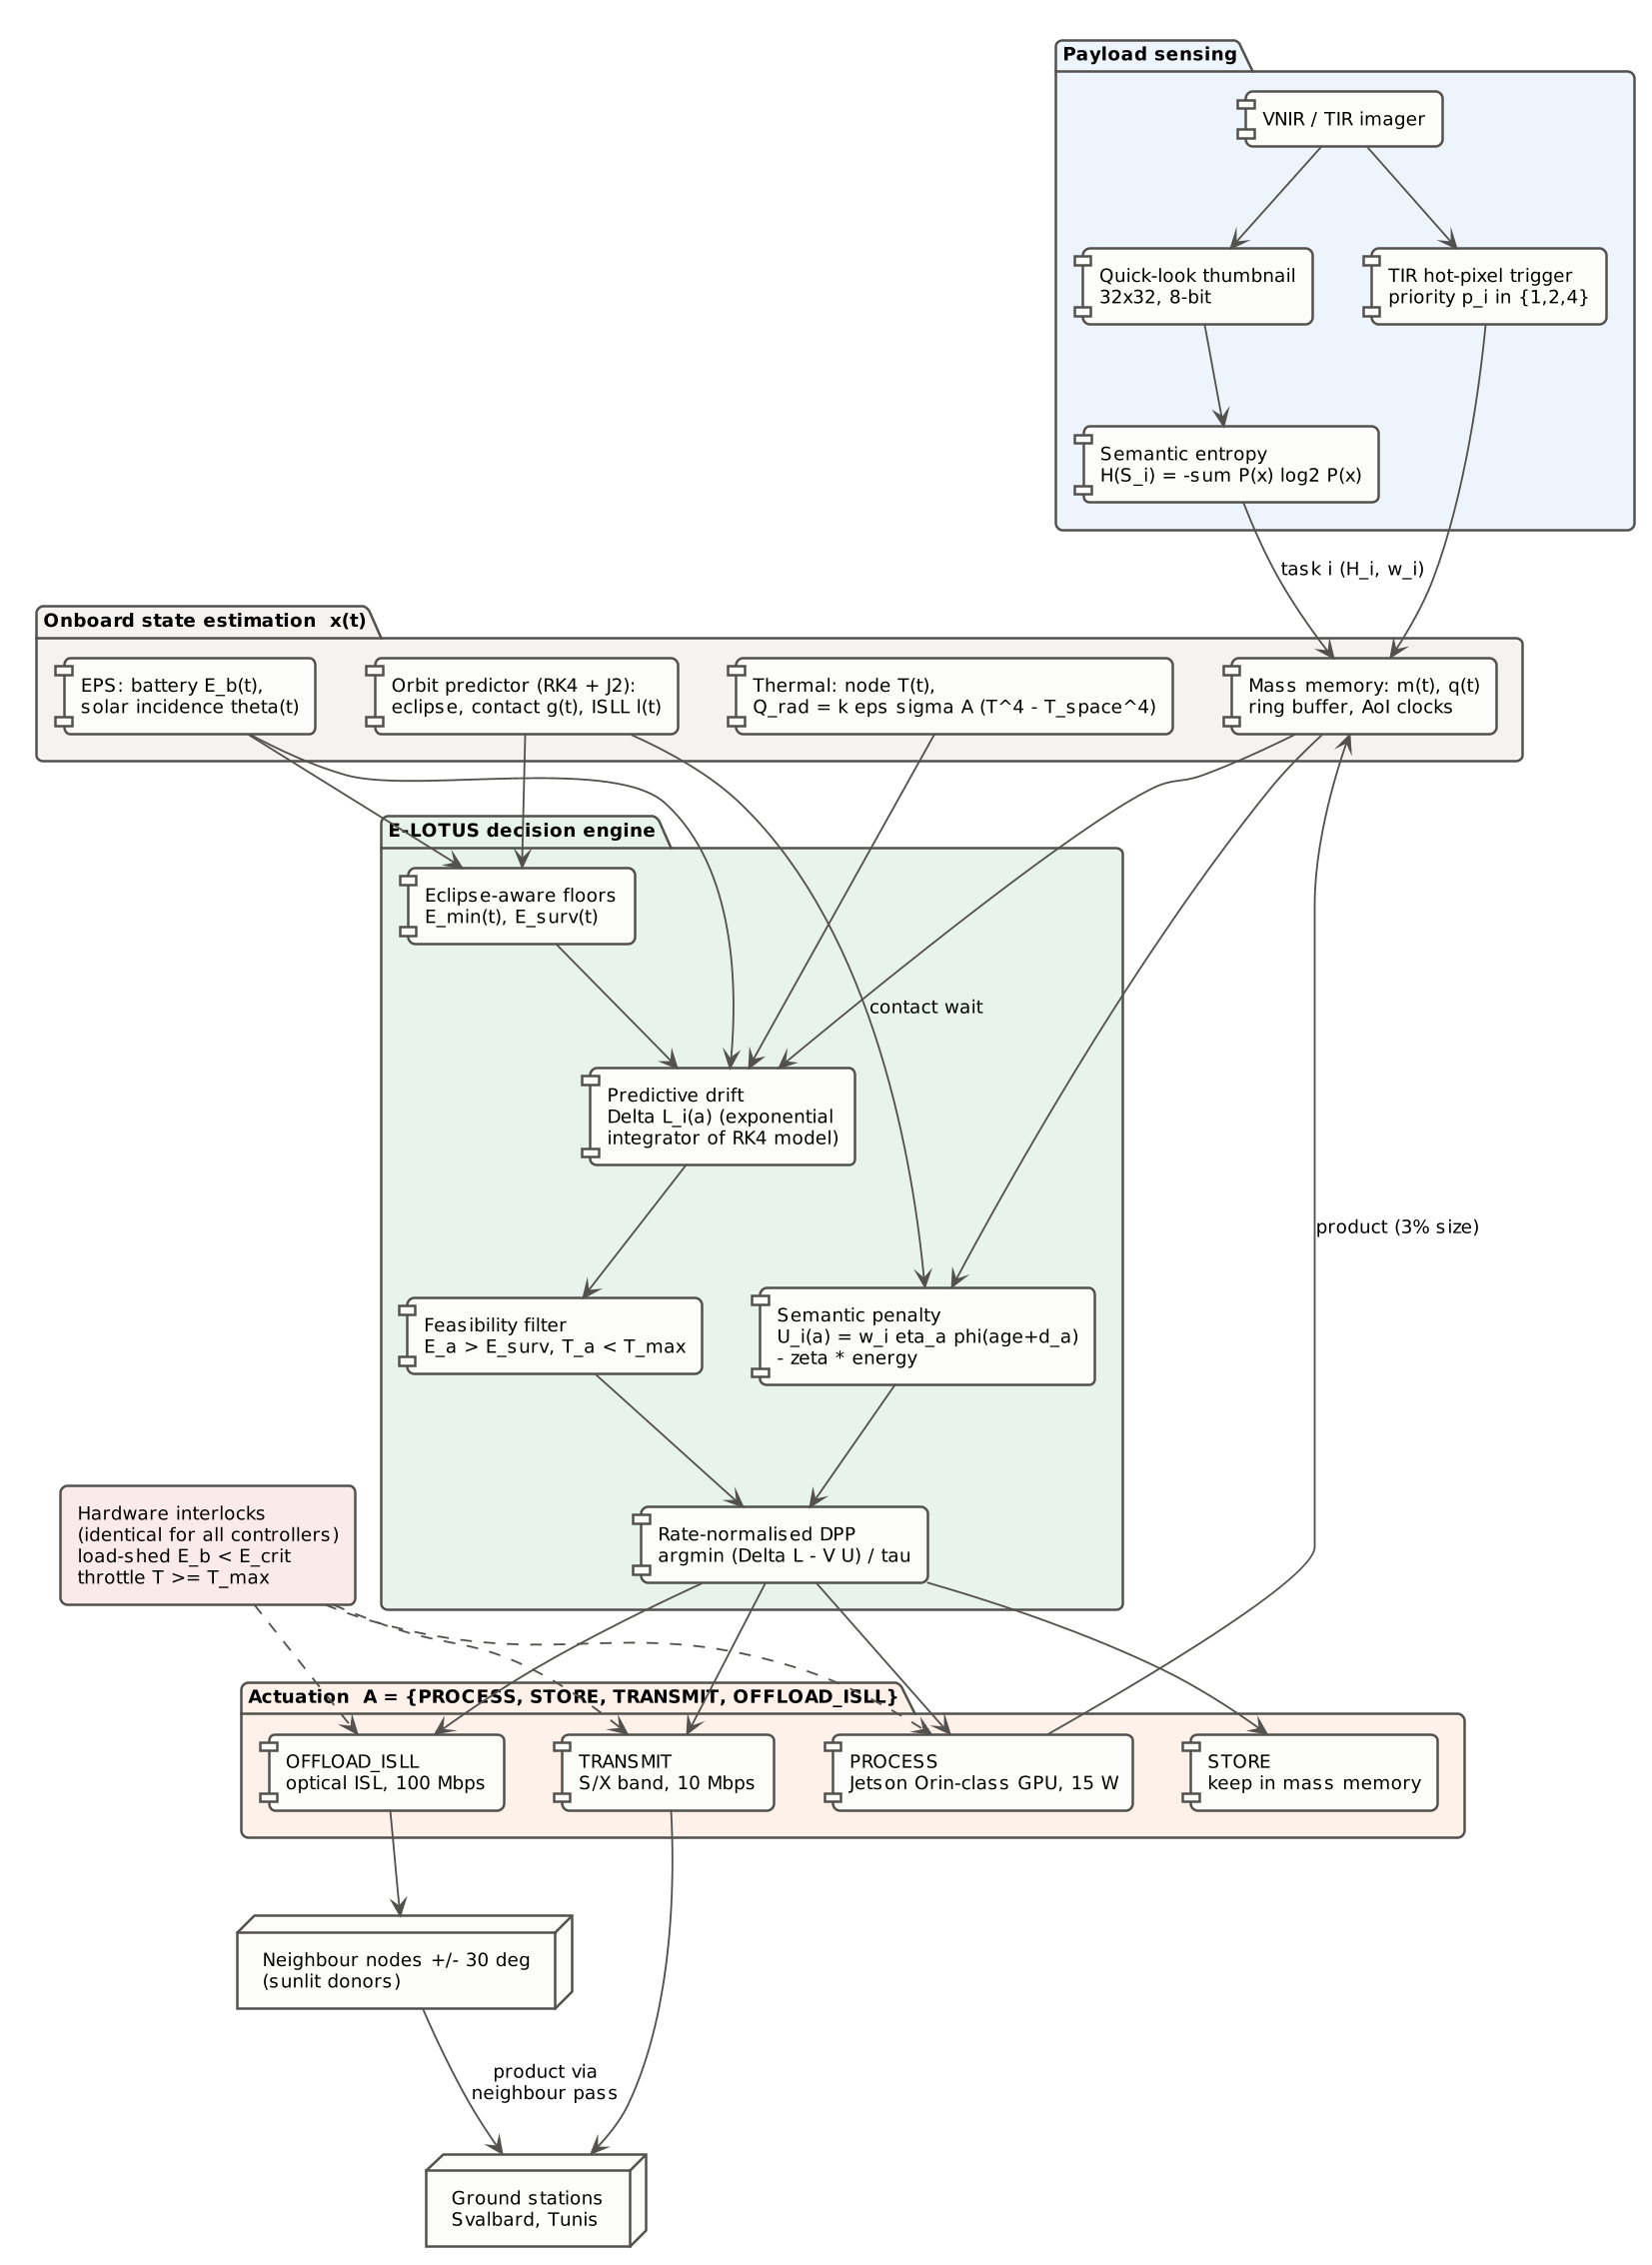
\includegraphics[width=\columnwidth]{fig1_architecture.png}
\caption{E-LOTUS system architecture (PlantUML source in the supplementary \texttt{diagrams/} folder). The engine fuses payload semantics, onboard state and the predicted orbit into one drift-plus-penalty score. Hardware interlocks sit below every controller.}
\label{fig:arch}
\end{figure}

\begin{figure}[t]
\centering
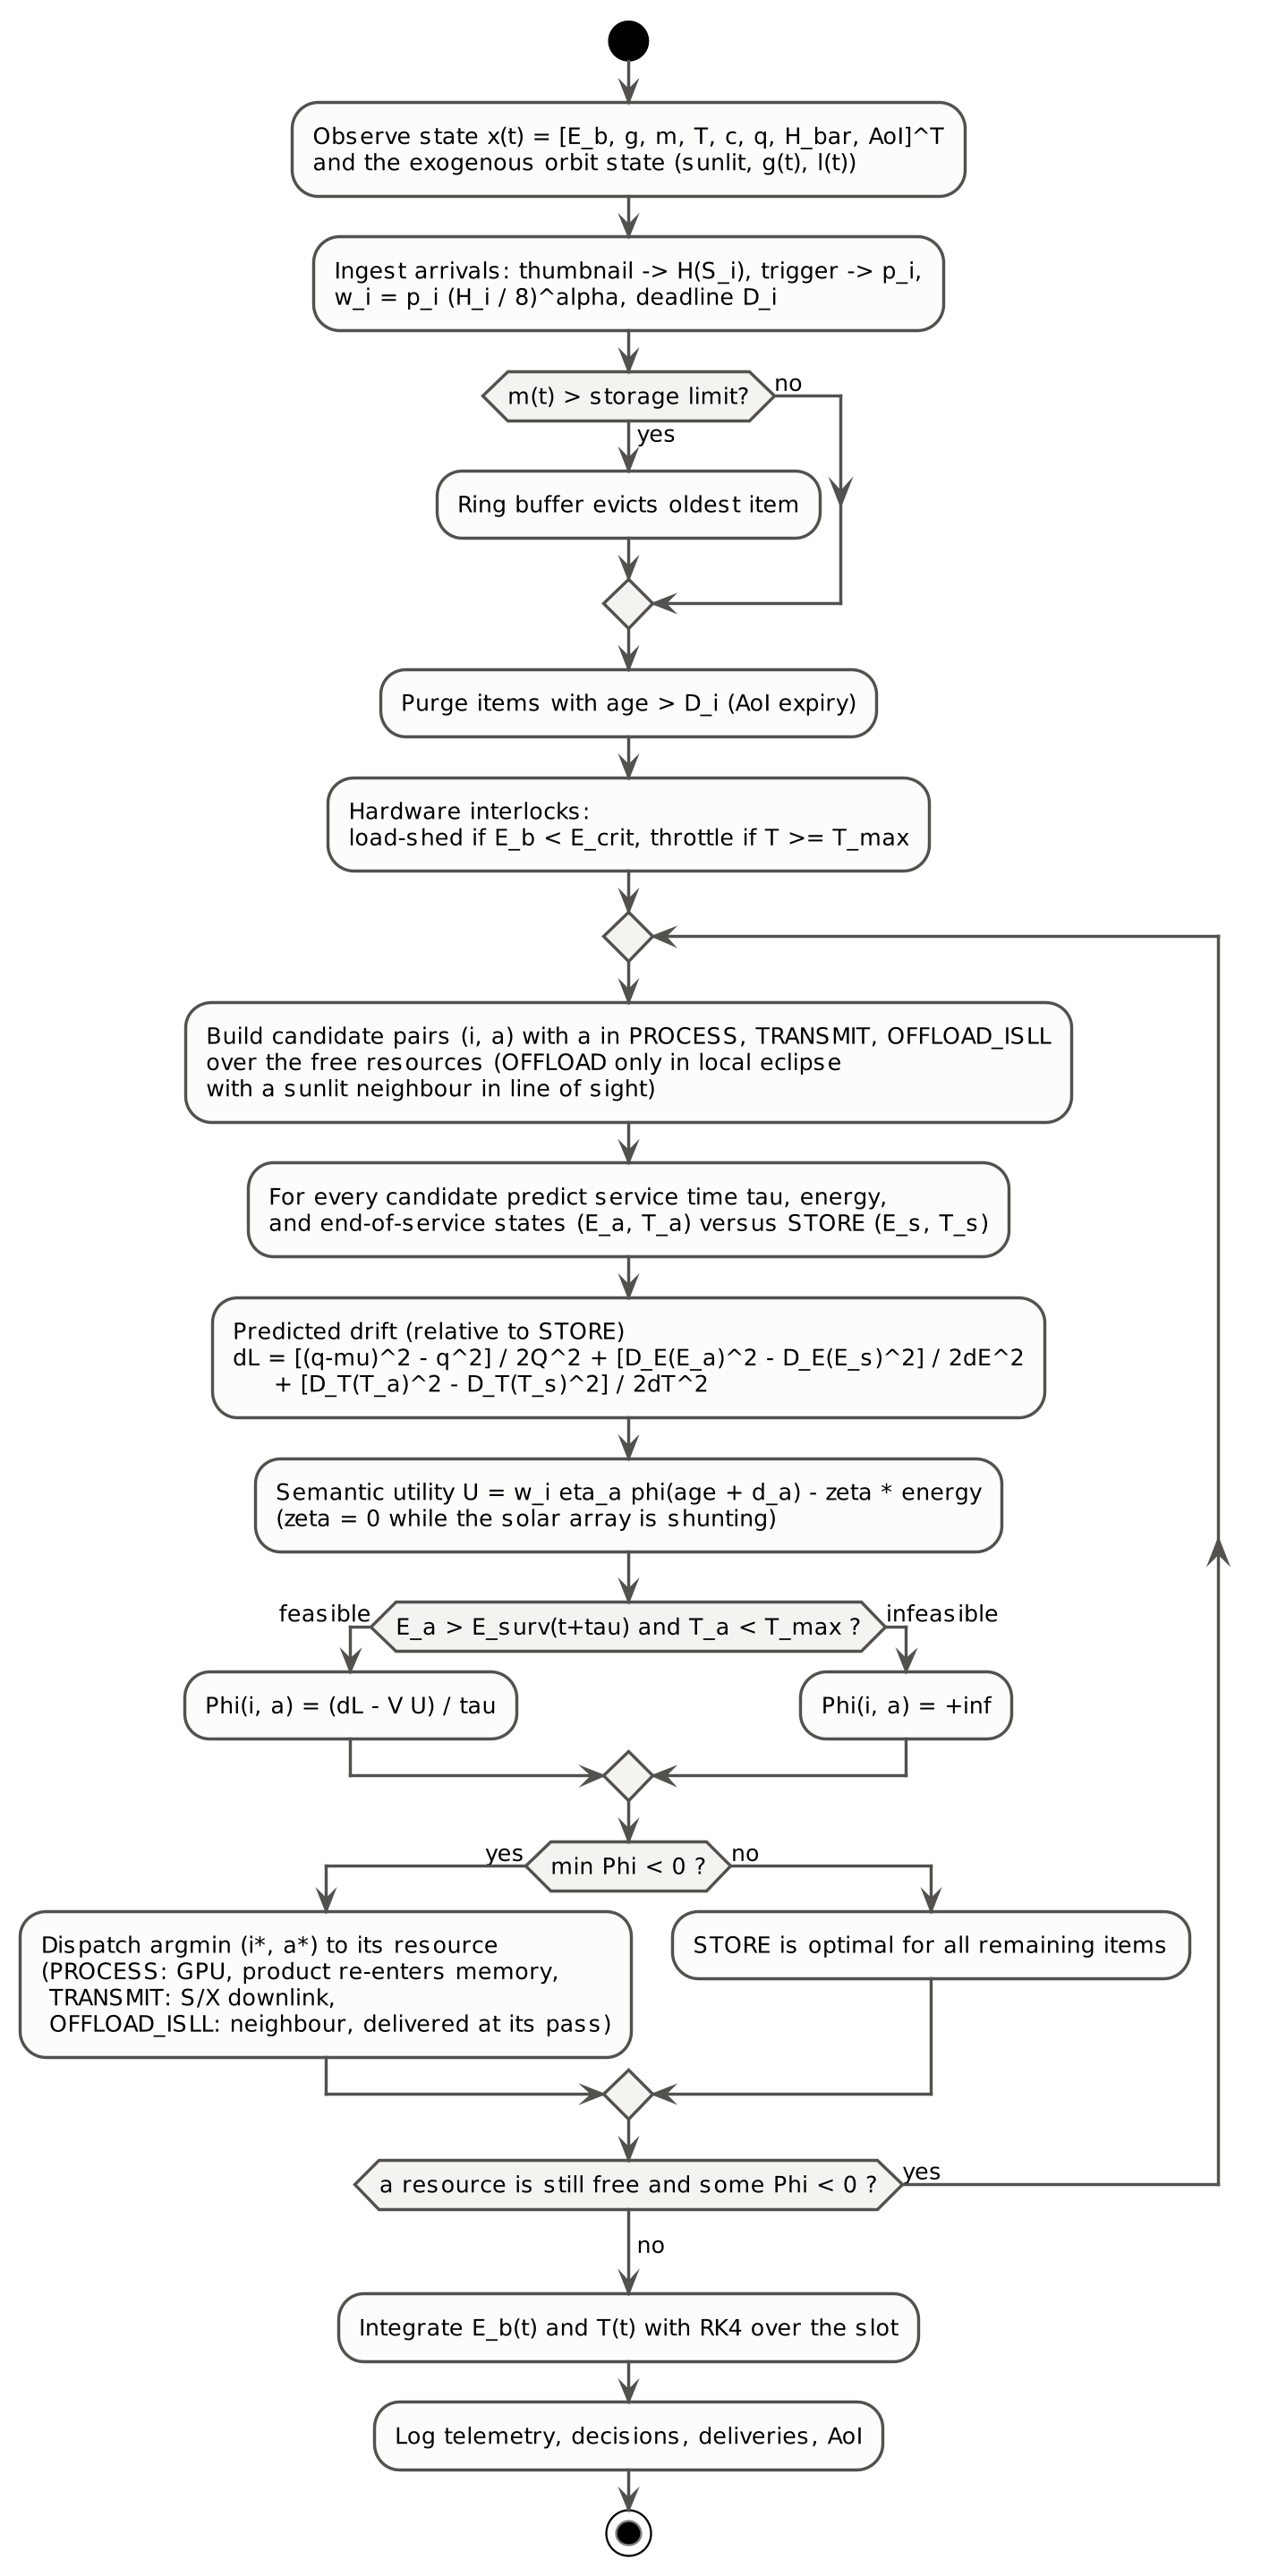
\includegraphics[width=0.80\columnwidth]{fig2_decision_flow.png}
\caption{Multi-objective decision flow executed in every \SI{10}{s} slot.}
\label{fig:flow}
\end{figure}

%=====================================================================
\section{Experiments and Roadmap}\label{sec:exp}
%=====================================================================
\subsection{Real-data testbed}\label{sec:data}
\textbf{Earth data.} We sample real NASA products along $\Phi$-sat-2's ground track through the Global Imagery Browse Services (GIBS)~\cite{gibs}. For each of the 30 days, global daily mosaics are retrieved at $4096\times2048$ pixels ($\approx$9.8~km/pixel), and every 30~s (\AtlasN\ sub-satellite points) a $32\times32$-pixel block ($\approx$313~km, comparable to one wide-swath scene) is cut around the sub-satellite point. From each block we record the following.
(i)~The Shannon entropy of the luminance of the VIIRS NOAA-20 corrected-reflectance true-colour image. This is the optical quick-look, used while the node is sunlit.
(ii)~The same entropy for the VIIRS I5 (11.45~$\mu$m) night brightness temperature. This is the thermal-IR quick-look, used in eclipse.
(iii)~The number of VIIRS 375~m active-fire pixels~\cite{schroeder2014viirs}.
(iv)~The MODIS Aqua cloud fraction~\cite{platnick2017modis}, decoded with the GIBS colour map.
(v)~The OpenStreetMap land fraction.
The sampler runs in a web browser and is released with the paper (\texttt{data/gibs\_sampler.js}).

\textbf{Workload.} The instrument acquires in strip mode as a Poisson process: one scene per \SI{45}{s} in sunlight (optical and thermal IR) and one per \SI{120}{s} in eclipse (thermal IR only). Each scene takes the real features of the nearest 30-s sample. Scene sizes (log-normal, \SI{50}{MB} median) and the processing cost (Table~\ref{tab:params}) are payload assumptions. The onboard thermal-IR trigger flags an alert ($p_i=4$, 90-min deadline) when the scene holds $\ge$\FireThr\ VIIRS fire pixels; this happens for \AlertRate\% of scenes. The hidden ground-truth value is $w_i^{\rm true}=3$ for alerts and $0.02+0.63\,\ell_i(1-c_i)$ otherwise, where $\ell_i$ is the real land fraction and $c_i$ the real cloud fraction. Clear land is therefore worth up to 0.65 and cloud or ocean about 0.02. The engine sees only $H_i$ and $p_i$. Over the 30 days the scene mix is \ShareOcean\% clear ocean, \ShareCloud\% cloudy, \ShareCoast\% coast, \ShareLand\% clear land and \ShareFire\% fire. On board this yields $\approx$\GenPerDay\ scenes and \RawGBDay~GB of raw data per day, against \DlGBDay~GB/day of downlink capacity. Processing everything would require \DemandDuty\% GPU duty, which the energy and thermal budgets cannot sustain.

\textbf{What real data say about entropy.} Fig.~\ref{fig:real}(b) shows that raw entropy does not separate value on real imagery. At quick-look scale, cloud fields are the \emph{most} textured scenes (median $H=\HCloud$~bit/px), above clear land (\HLand) and partly cloudy ocean (\HOcean). Their rank correlation with ground-truth value is only $\rho=\RhoRawOpt$ for optical quick-looks and $\rho=\RhoRawTir$ for thermal-IR ones. Within land scenes, entropy is even \emph{anti}-correlated with the clear-sky fraction ($\rho=\RhoWithinOpt$ optical, $\RhoWithinTir$ thermal IR), because broken cloud adds texture. The procedural thumbnails of our first draft assumed flat, low-entropy clouds, and the real data refute that assumption. We therefore designed \eqref{eq:west} on the first \HalfDays\ days and evaluated it on the held-out last \HalfDays\ days (Fig.~\ref{fig:real}(c)). Ranked by raw entropy, the top 30\% of scenes hold only \CapRaw\% of the value, worse than random (\CapRandom\%). The land prior alone reaches \CapLand\%, and the E-LOTUS estimator reaches \CapEL\% ($\rho=\RhoEL$), against \CapOracle\% for a label-aware oracle. Cloud screening on board, for example with a CloudScout-type network~\cite{giuffrida2022phisat}, would close most of the remaining gap and is planned for Phase~3.

\begin{figure*}[t]
\centering
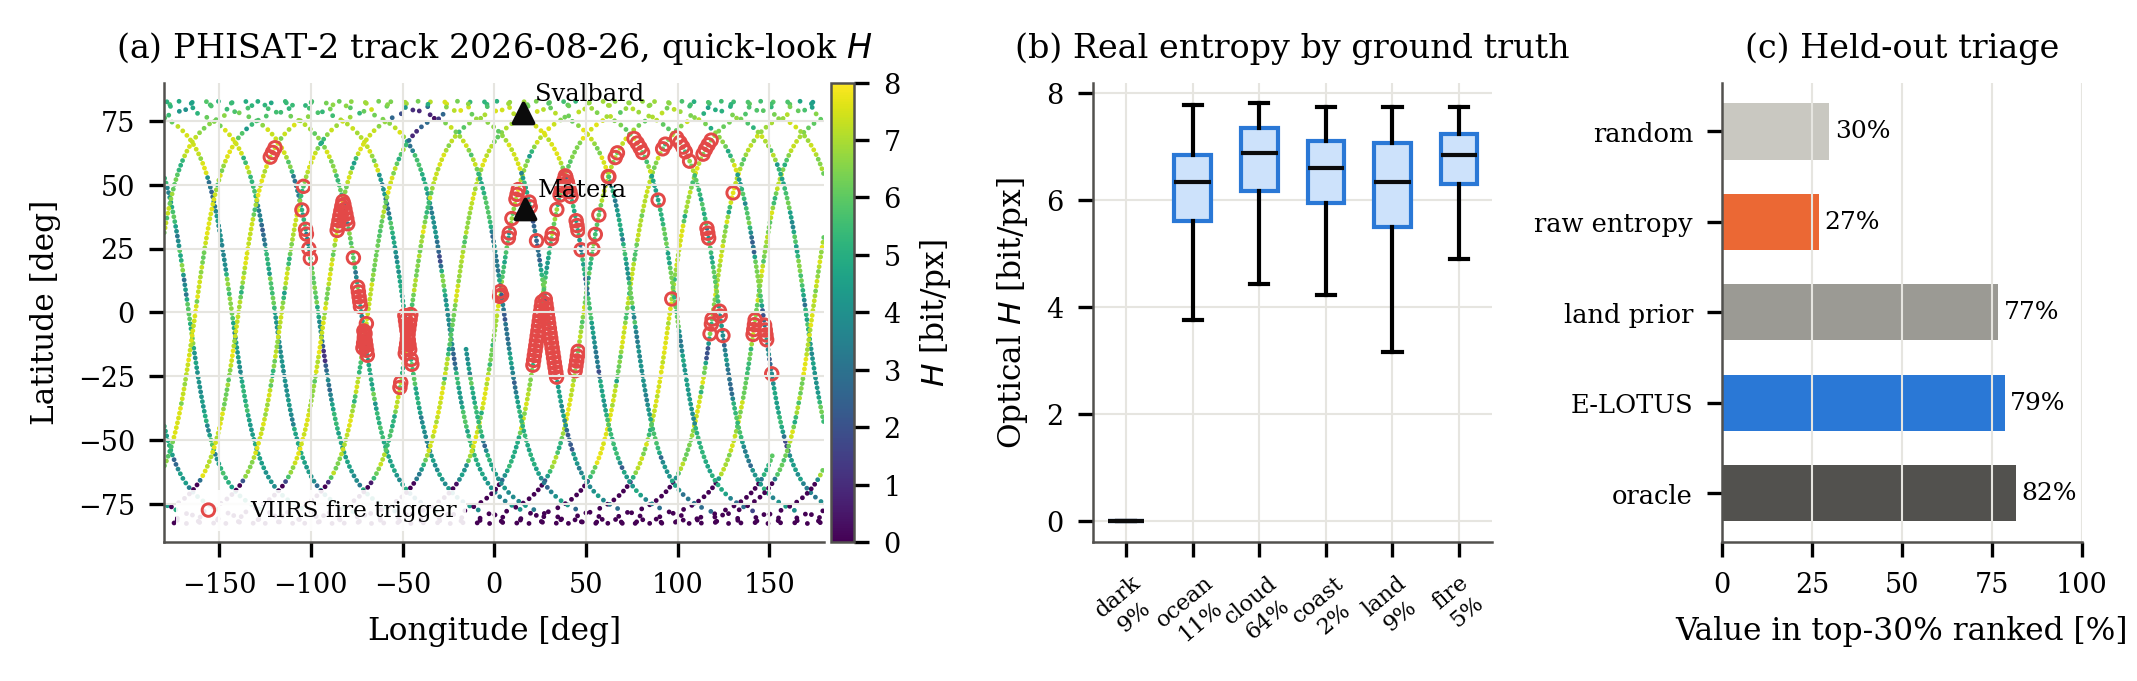
\includegraphics[width=\textwidth]{fig3_realdata.png}
\caption{Real data. (a)~The $\Phi$-sat-2 ground track on the first day of the window (SGP4 on the real TLE). Colour shows quick-look entropy (VIIRS true colour when sunlit, I5 brightness temperature in eclipse); red circles mark scenes that fire the thermal-IR trigger (VIIRS 375~m detections: African, South American and Siberian fire belts). (b)~Optical quick-look entropy by ground-truth class over \Days\ days, with class shares. (c)~Share of the ground-truth value found in the top 30\% of scenes on the held-out days, for each ranking.}
\label{fig:real}
\end{figure*}

\textbf{Controllers.} Every controller sees the identical arrival stream and identical hardware interlocks: load-shed below $E_{\rm crit}=\SI{20}{Wh}$ and GPU throttle above $T_{\max}=\SI{60}{\celsius}$. The four baselines are the following.
\emph{Always-Transmit} downlinks raw data in FIFO order.
\emph{Greedy-Process} processes in FIFO order whenever the GPU is free and downlinks products.
\emph{Store-and-Forward} buffers everything and forwards by (priority, entropy) during passes.
\emph{Rule-Based} is a deliberately strong entropy-aware rule engine. It processes the highest-$\hat w$ item if SOC$\ge$50\% and $T<T_{\rm safe}$, downlinks products first, and offloads during eclipse.
We selected $V=0.3$ and $\zeta=0.5$ on a separate synthetic tuning trace. The main run uses seed 2026 over all \Days\ real days. The robustness study uses 24-h windows on different real days with seeds 1--5.

\begin{table}[t]
\centering
\caption{Simulation parameters}\label{tab:params}
\footnotesize
\begin{tabular}{@{}p{0.24\columnwidth}p{0.70\columnwidth}@{}}
\toprule
Orbit & PHISAT-2 (NORAD 60470), CelesTrak TLE epoch 2026-09-26, SGP4, $\Delta t=10$ s\\
Altitude / period & \AltMin--\AltMax\ km, $i=\TleInc^\circ$, $T=\PeriodMin$ min, eclipse $\le$\EclMax\ min\\
Ground stations & KSAT SvalSat, ASI Matera; mask $10^\circ$; \ContactMin\ min/day\\
Earth data & NASA GIBS daily VIIRS/MODIS, \DateStart\ to \DateEnd, 313 km quick-look blocks\\
Battery & 100 Wh LiFePO$_4$, $\eta_c=\eta_d=0.95$, $P_{\rm ch}\le40$ W\\
Floors & $E_{\rm crit}=20$ Wh, $E_{\rm res}=30$ Wh (+ eclipse term)\\
Solar array & 3 body faces $\times$ 20 W at normal incidence\\
Loads & bus 5 W; GPU 1.5/15 W; TX 12 W; ISL 8 W\\
Compute & Jetson Orin-class, 1000 GFLOP/s eff.; 900 GFLOP/MB\\
Product & $\kappa=0.03$, $\eta_p=0.9$\\
Radiator & $\epsilon=0.85$, $A=0.045$ m$^2$, $C=1500$ J/K\\
Thermal limits & $T_{\rm safe}=45^\circ$C (soft), $T_{\max}=60^\circ$C (throttle)\\
Env. heat & $Q_{\rm sun}=6$ W (sunlit), $Q_{\rm IR}=3$ W\\
Links & S/X 10 Mbps; optical ISL 100 Mbps, neighbours $\pm30^\circ$\\
Donor model & 400 GFLOP/s spare, 60 TFLOP bucket\\
Storage & 8 GB ring buffer\\
Deadlines & alert 90 min, routine 12 h\\
E-LOTUS & $V=0.3$, $\zeta=0.5$, $\alpha=3$, $\varepsilon=0.1$, $\Delta E=5$ Wh, $\Delta T=5$ K\\
\bottomrule
\end{tabular}
\end{table}


\subsection{Metrics}
The metrics follow the challenge's evaluation criteria. \emph{Decision quality} is the delivered semantic value $\sum_i w_i^{\rm true}\phi_i$ and its share of a \emph{contact-limited ceiling}. The ceiling is the value obtained if every item reached the ground at the first pass after its generation, with unlimited compute, energy and bandwidth; no controller can exceed it. We also report the \emph{completion rate} (items whose information reached the ground), \emph{payload energy}, mean delivery \emph{latency} and ground AoI, and \emph{resource utilisation} (GPU duty and downlink utilisation), together with the minimum SOC, the maximum temperature, and the load-shed and throttle time.

\subsection{Long-horizon results}
Table~\ref{tab:main} summarises the \Days-day run on real data. E-LOTUS delivers \ELvalueDay\ units of semantic value per day, which is \ELceil\% of the contact-limited ceiling of \CeilDay/day. It never load-sheds and never throttles.

\emph{Naive baselines.} Always-Transmit and Store-and-Forward leave the GPU idle and can move only \DlGBDay~GB/day of the \RawGBDay~GB/day produced, so most data is overwritten in the ring buffer. On real imagery this is severe. Two thirds of the scenes are cloudy, so FIFO downlink of raw data (Always-Transmit) returns only \ATvalueDay/day, and E-LOTUS delivers $\ELvalueGainAT\times$ more. Store-and-Forward forwards by priority, which saves most alerts (\SFalerts\% on time) and gives the lowest latency (\SFlat~min), but E-LOTUS still delivers $\ELvalueGainSF\times$ its value.

\emph{Greedy-Process collapses.} It averages only \GPvalueDay/day and spends \GPshed\% of the time load-shed. Running the GPU in FIFO order through sunlit arcs drives the node to $T_{\max}$ (\GPtmax\,$^\circ$C). The same policy then drains the battery to the hard floor (SOC$_{\min}$ \GPsocmin\%), after which the node oscillates between shedding and recovery. Under overload, FIFO service also means the oldest items are processed first, and those items are closest to expiry, so their products miss their AoI deadlines before the next pass.

\emph{Strong rule engine.} Rule-Based uses the same value estimate \eqref{eq:west} and the same ISL, so it isolates what the Lyapunov machinery adds. E-LOTUS delivers \ELvalueGainRB\% more value and \ELcomplDelta~percentage points higher completion (\ELcompl\% vs.\ \RBcompl\%), with \ELovfRed\% fewer ring-buffer overwrites. It does so by spending \ELenergyDeltaPct\% more payload energy (\ELenergy\ vs.\ \RBenergy~Wh/day). Both controllers keep the battery above 65\% (SOC$_{\min}$ \ELsocmin\% vs.\ \RBsocmin\%), so the extra energy is solar input that the rule engine's fixed thresholds leave unused. The costs are a warmer node (\ELtmax\ vs.\ \RBtmax\,$^\circ$C, since the thermal deficit is soft by design and $T_{\max}$ is never approached) and a longer mean latency (\ELlat\ vs.\ \RBlat~min). The latency difference arises because E-LOTUS processes, and later delivers, many routine scenes that the rule engine simply lets expire. Alert delivery is the same for both (\ELalerts\% vs.\ \RBalerts\% on time), because it is bounded by pass geometry.

Fig.~\ref{fig:telemetry} shows the mechanism over the first real day. Greedy-Process saturates the radiator in sunlight and then drains the battery. E-LOTUS instead holds $T$ near $T_{\rm safe}$ by interleaving \textsc{Process} with \textsc{Store}, spends the stored heat margin during eclipse, and moves work to the neighbours (green) at the ends of each eclipse, when a donor is sunlit.

\begin{figure*}[t]
\centering
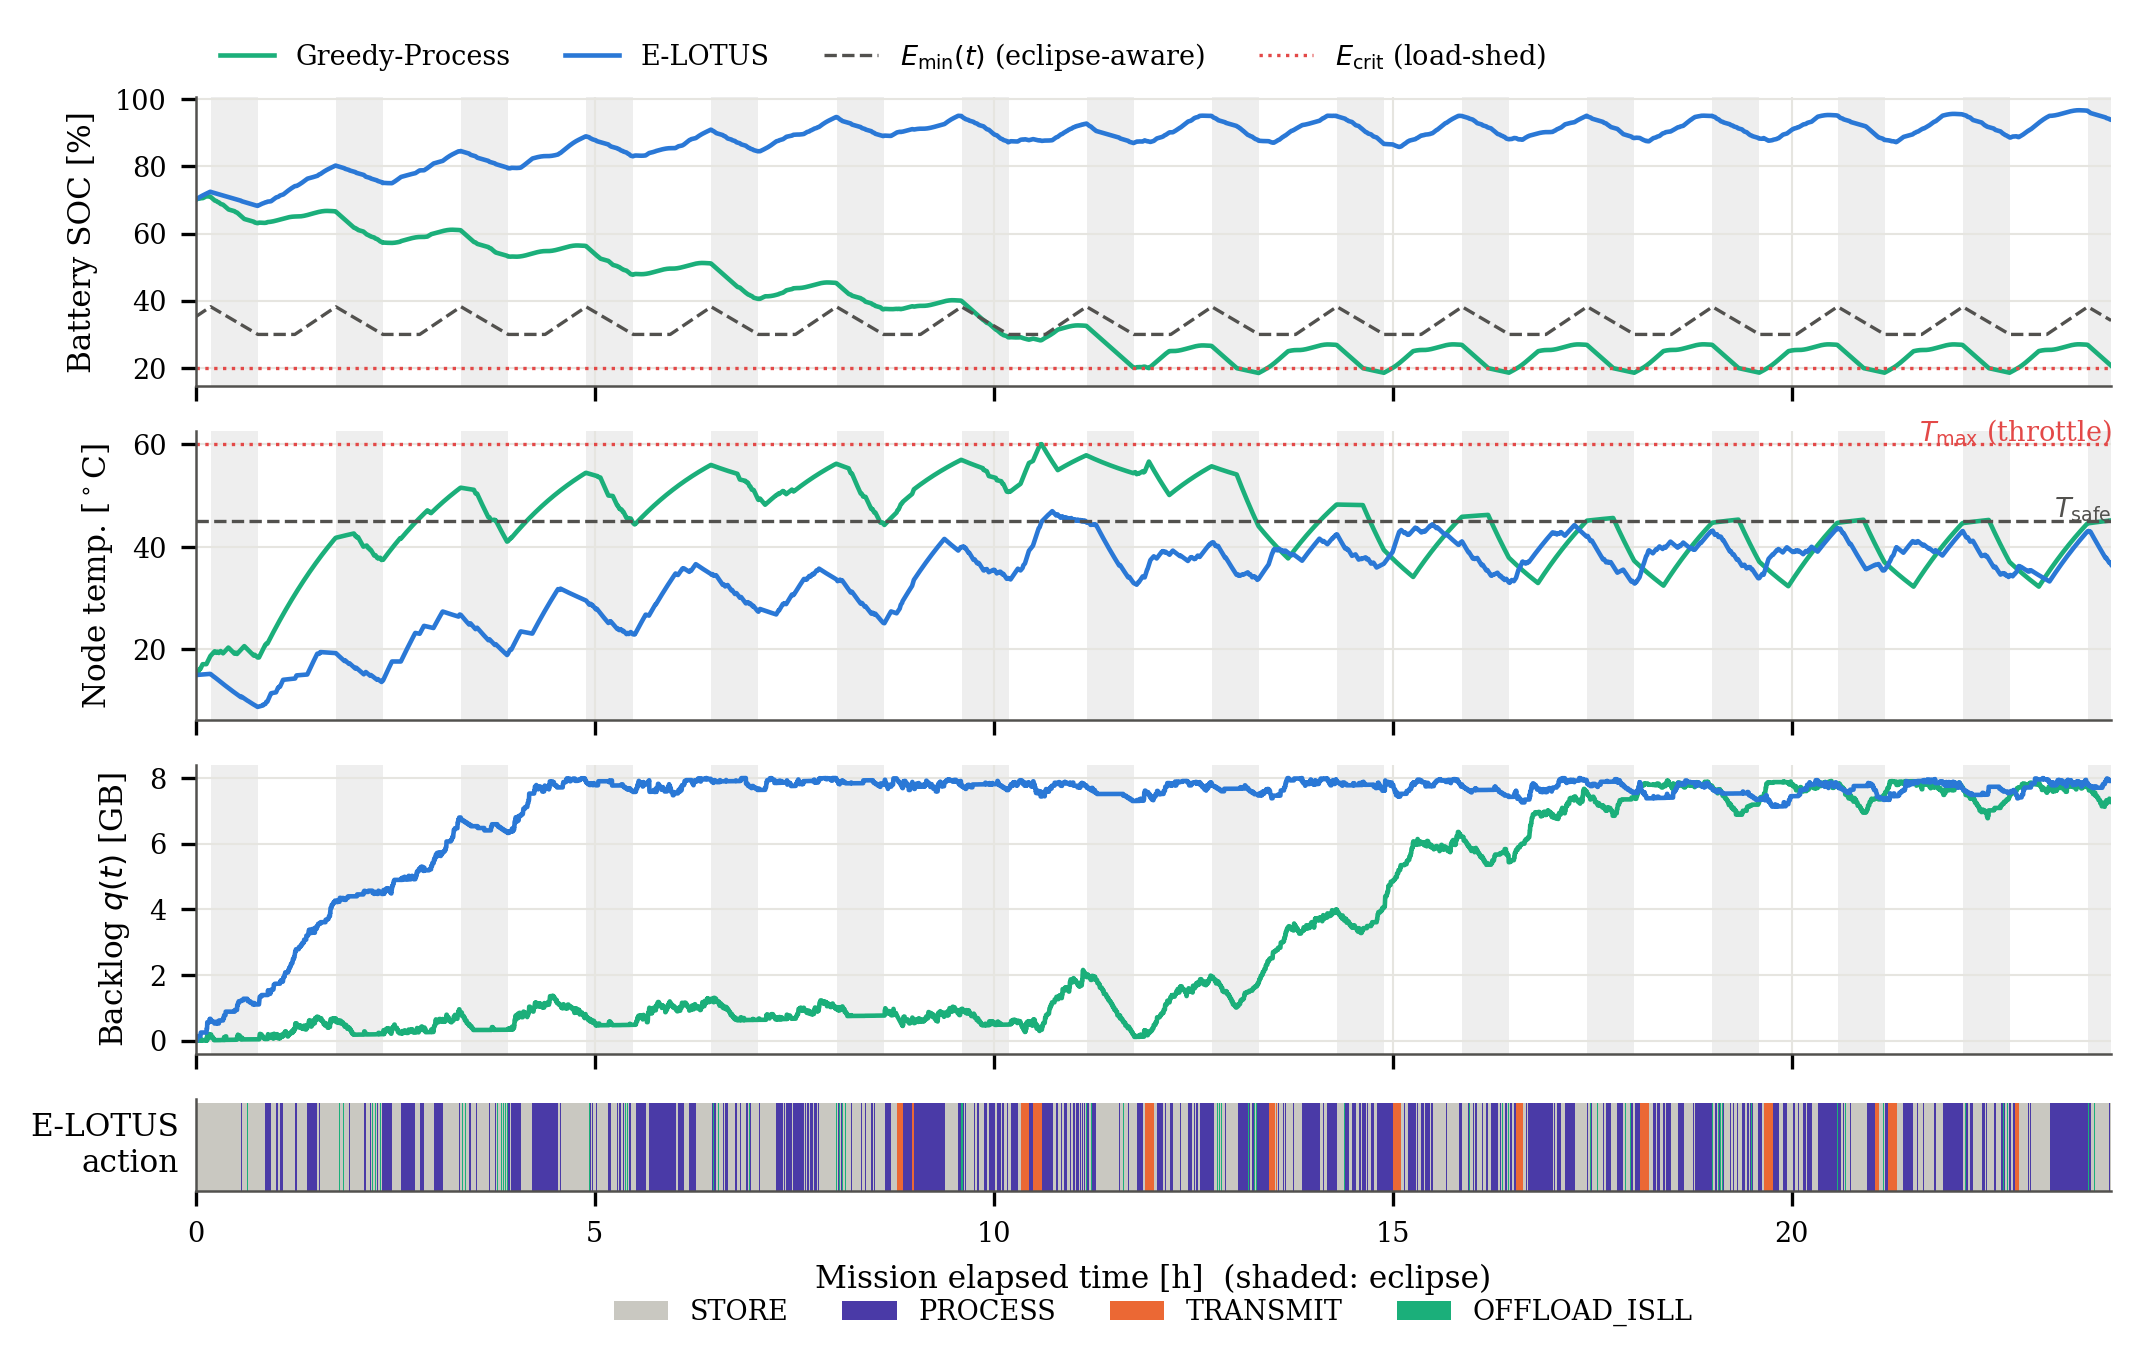
\includegraphics[width=\textwidth]{fig4_telemetry.png}
\caption{First 24~h of the main run (real orbit and real scenes of \DateStart). Shaded bands mark eclipse. Top to bottom: battery SOC with the eclipse-aware floor $E_{\min}(t)$ and the load-shed threshold; node temperature; backlog $q(t)$; action taken by E-LOTUS.}
\label{fig:telemetry}
\end{figure*}

\begin{table*}[t]
\centering
\caption{20-day benchmark (seed 2026): per-day averages. Ceiling = contact-limited upper bound (176.4 value/day). Best in bold.}\label{tab:main}
\footnotesize
\setlength{\tabcolsep}{3.1pt}
\begin{tabular}{@{}lrrrrrrrrrrrrr@{}}
\toprule
Controller & Value/day & \% ceil. & Compl.\,\% & Alerts\,\% & Energy Wh/d & Value/Wh & Lat.\,min & SOC$_{\min}$\,\% & $T_{\max}$\,$^\circ$C & Shed\,\% & GPU\,\% & DL\,\% & Ovf./d\\
\midrule
\textbf{E-LOTUS (ours)} & \textbf{152.1} & \textbf{86.2} & \textbf{83.2} & 75.5 & 217 & 0.70 & 160 & 68 & 49.7 & 0.0 & 51 & 84 & 213\\
Rule-Based & 144.0 & 81.6 & 49.7 & \textbf{75.6} & 161 & 0.90 & 133 & 66 & 45.3 & 0.0 & 33 & 100 & 713\\
Store-and-Forward & 72.7 & 41.2 & 7.5 & 64.3 & 52 & \textbf{1.40} & 77 & 68 & 15.2 & 0.0 & 0 & 100 & 1324\\
Always-Transmit & 3.4 & 1.9 & 7.4 & 0.0 & 52 & 0.07 & 165 & 68 & 15.2 & 0.0 & 0 & 100 & 1284\\
Greedy-Process & 5.7 & 3.2 & 10.1 & 1.8 & 219 & 0.03 & 543 & 18 & 60.1 & 39.0 & 60 & 4 & 325\\
\bottomrule
\end{tabular}
\end{table*}


\begin{figure}[t]
\centering
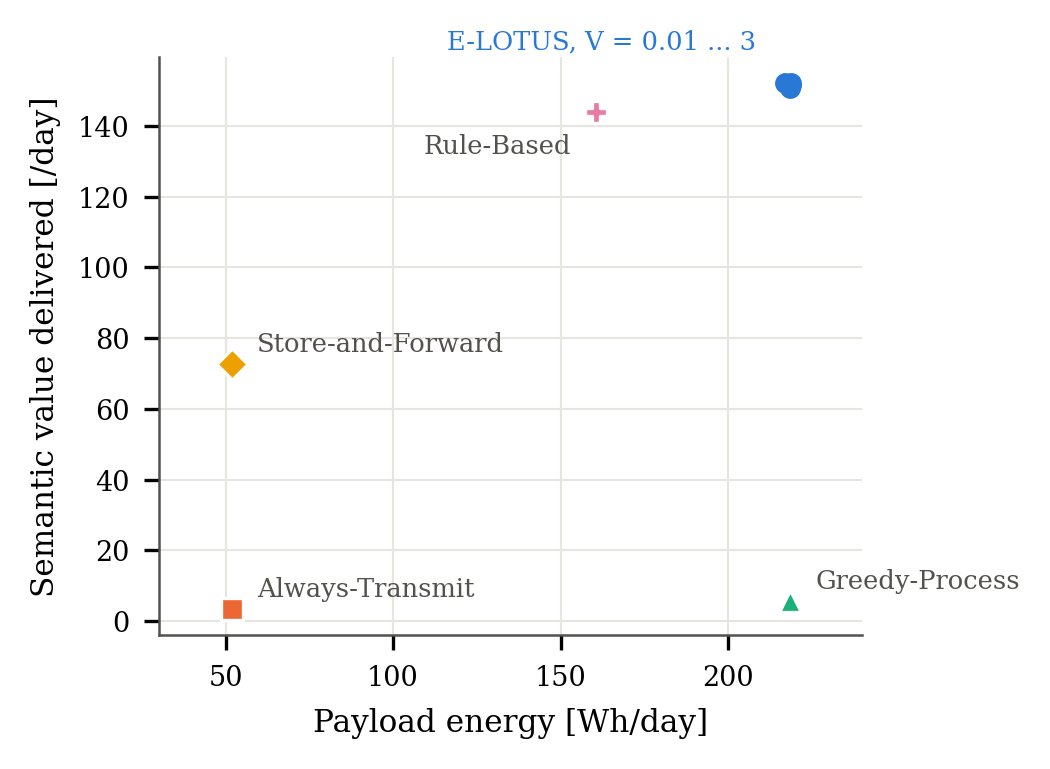
\includegraphics[width=\columnwidth]{fig5_pareto.png}
\caption{Value versus payload energy (\Days-day per-day averages, real data). The E-LOTUS family ($V\in[0.01,3]$) delivers the most value. Store-and-Forward is the most frugal, and Greedy-Process spends the same energy as E-LOTUS for almost no value.}
\label{fig:pareto}
\end{figure}

\begin{figure}[t]
\centering
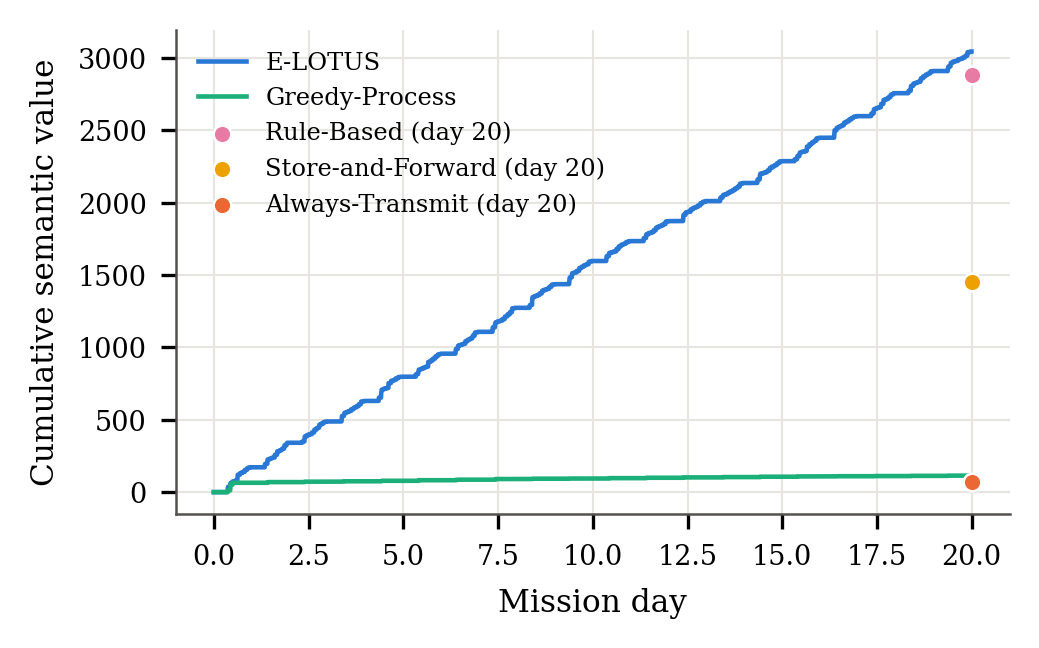
\includegraphics[width=\columnwidth]{fig7_cumulative.png}
\caption{Cumulative delivered semantic value over the \Days-day real-data run.}
\label{fig:cum}
\end{figure}

\subsection{Effect of the trade-off parameter $V$}
Fig.~\ref{fig:vsweep} sweeps $V$ over two and a half decades. The net utility $\bar U-\zeta\bar{\mathcal E}$ rises from \VnetLo\ per day at $V=0.01$ to a plateau of about \VnetHi\ for $V\ge0.3$. On the plateau it varies by less than 3\%, which is within the effect of the greedy multi-resource fill. The mean backlog grows monotonically from \VqLo\ to \VqHi~GB. Both trends are consistent with the $[O(1/V),O(V)]$ prediction of Theorem~\ref{thm:dpp}. They are compressed because long-run energy is set by the harvest and the backlog saturates near the 8~GB storage limit. The clearest effect of $V$ is on the battery. For $V\le0.1$ the queue term dominates and E-LOTUS draws the battery down to its eclipse-aware floor (SOC$_{\min}$ \VsocLo\%). For $V\ge0.3$ the SOC never falls below \VsocHi\%. Operators can therefore choose the depth of discharge with one number.

\begin{figure*}[t]
\centering
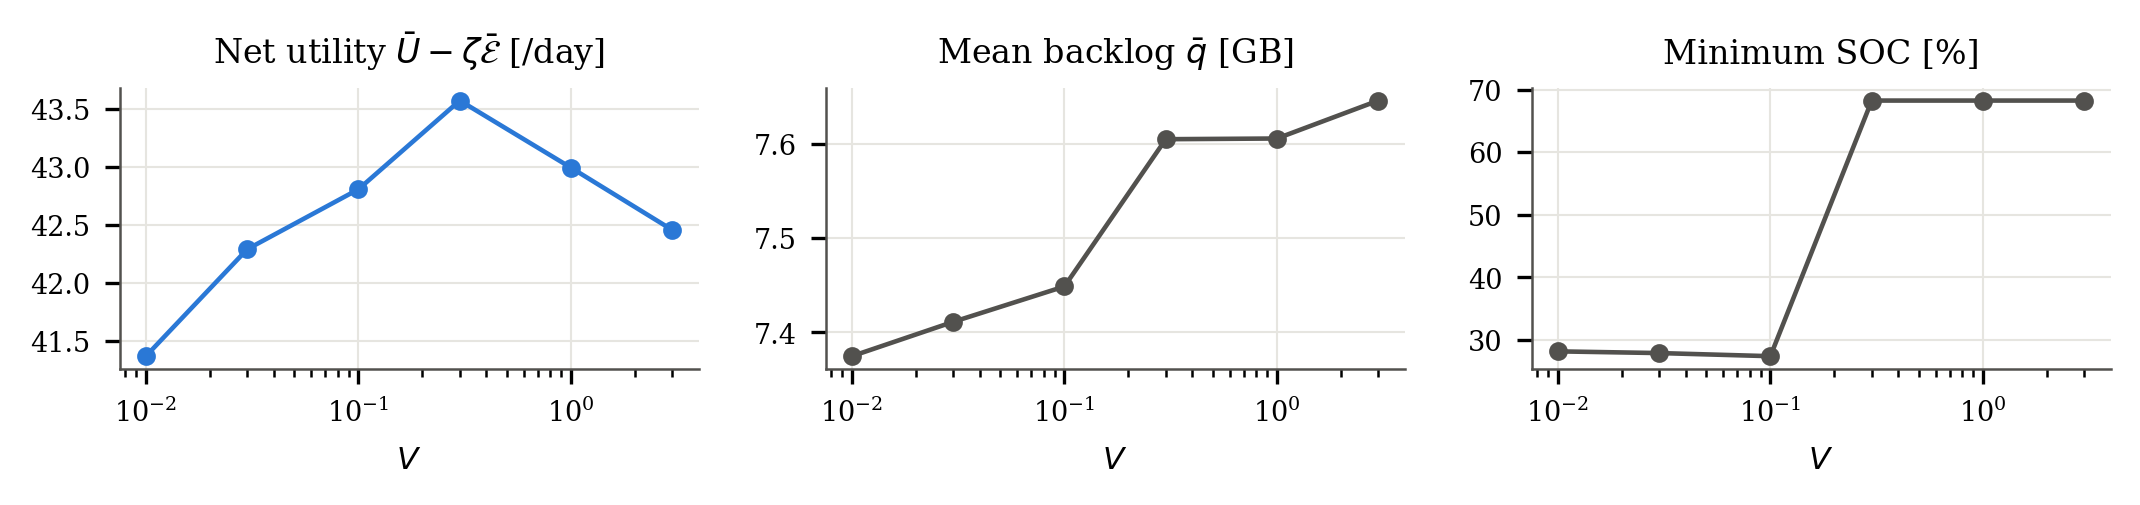
\includegraphics[width=0.92\textwidth]{fig6_vsweep.png}
\caption{Sweep of the Lyapunov trade-off parameter $V$ (\Days\ real days each).}
\label{fig:vsweep}
\end{figure*}

\subsection{Ablations}
Table~\ref{tab:abl} removes one component at a time.

\emph{The value estimator} matters most. With priority flags only, value falls by \NoEntdrop\%. With raw entropy and no land prior, which was our original design, value falls by \Rawdrop\%. In both cases the engine spends energy on bright, textured cloud scenes, and the SOC drops to about \Rawsocmin\%, just above the load-shed threshold, with the node reaching \Rawtmax\,$^\circ$C. The land prior is therefore worth +\RawGainEL\% of value on real data.

\emph{ISL offload}: removing it lowers value by \NoISLdrop\% (\NoISLvalue\ vs.\ \ELvalueDay/day), lowers completion from \ELcompl\% to \NoISLcompl\%, and raises overwrites from \ELovf\ to \NoISLovf\ per day.

\emph{Eclipse-aware floors} leave results unchanged at $V=0.3$, where the battery never approaches them. At $V=0.01$, where the battery is drawn down, static floors deliver \StaticLowVvalue/day against \LowVvalue/day with eclipse-aware floors, a \StaticLowVdrop\% loss. The floors thus act as protection that engages only when it is needed.

\begin{table}[t]
\centering
\caption{Ablations (20 days, per-day averages)}\label{tab:abl}
\footnotesize
\setlength{\tabcolsep}{1.6pt}
\begin{tabular}{@{}lrrrrrr@{}}
\toprule
Variant & Value/d & Compl.\% & Wh/d & SOC$_{\min}$ & $T_{\max}$ & Shed\%\\
\midrule
E-LOTUS (full, $V$=0.3) & 152.1 & 83.2 & 217 & 68 & 49.7 & 0.0\\
\quad w/o ISLL offload & 149.1 & 71.7 & 217 & 68 & 49.6 & 0.0\\
\quad w/o entropy weighting & 127.0 & 78.1 & 222 & 20 & 54.1 & 0.0\\
\quad raw entropy only & 139.3 & 83.8 & 222 & 20 & 53.5 & 0.0\\
\quad static floors & 152.1 & 83.2 & 217 & 68 & 49.7 & 0.0\\
E-LOTUS, $V$=0.01 & 150.7 & 78.9 & 219 & 28 & 46.5 & 0.0\\
\quad static floors, $V$=0.01 & 148.0 & 77.9 & 221 & 33 & 46.6 & 0.0\\
\bottomrule
\end{tabular}
\end{table}


\subsection{Robustness}\label{sec:stress}
Table~\ref{tab:stress} repeats the comparison on 24-h windows over different real days with independent arrival seeds: five for the nominal case and three per stress scenario. Across the five nominal days, E-LOTUS delivers $\MSelValue\pm\MSelValueStd$ against $\MSrbValue\pm\MSrbValueStd$ for Rule-Based (+\MSgain\%). It completes \MScomplDelta~points more tasks with \MSenergyWord\ payload energy and \MSlatWord\ latency.

E-LOTUS delivers more value than Rule-Based in \StressWins\ of \StressN\ stress scenarios (gain between \StressGainMin\% and \StressGainMax\%), with completion gains between \StressComplMin\ and \StressComplMax\ points. With a degraded radiator ($k=0.75$), Greedy-Process is throttled \RadGPthr\% of the time. E-LOTUS exceeds the soft limit by design (\RadELtmax\,$^\circ$C), trading it against value, but never reaches $T_{\max}$. Rule-Based stays competitive in value wherever its hand-set thresholds happen to fit, but it has no mechanism to trade value against backlog, which shows up as consistently lower completion.

\begin{table*}[t]
\centering
\caption{Robustness over 24-h horizons: mean $\pm$ std over independent seeds (5 seeds nominal, 3 seeds per stress scenario)}\label{tab:stress}
\footnotesize
\setlength{\tabcolsep}{3.0pt}
\begin{tabular}{@{}llrrrrrrrr@{}}
\toprule
Scenario & Controller & Value & \% ceil. & Compl.\,\% & Energy Wh & SOC$_{\min}$\,\% & $T_{\max}$\,$^\circ$C & Shed\,\% & Thr.\,\%\\
\midrule
\multirow{3}{*}{Nominal (5 seeds)} & E-LOTUS & 155.5$\pm$10.2 & 85.5$\pm$0.8 & 71.3$\pm$2.4 & 193 & 69 & 46.1 & 0.0 & 0.0\\
 & Rule-Based & 148.9$\pm$9.8 & 81.9$\pm$1.1 & 48.3$\pm$1.2 & 162 & 68 & 42.6 & 0.0 & 0.0\\
 & Greedy-Process & 49.1$\pm$6.3 & 27.2$\pm$4.8 & 44.4$\pm$3.5 & 264 & 19 & 59.8 & 20.1 & 1.0\\
\midrule
\multirow{3}{*}{Load $\times1.5$} & E-LOTUS & 230.4$\pm$16.1 & 82.3$\pm$1.6 & 58.1$\pm$1.1 & 217 & 61 & 51.2 & 0.0 & 0.0\\
 & Rule-Based & 224.2$\pm$17.8 & 80.1$\pm$2.3 & 44.7$\pm$1.1 & 212 & 62 & 46.6 & 0.0 & 0.0\\
 & Greedy-Process & 19.0$\pm$11.4 & 7.0$\pm$4.4 & 18.8$\pm$7.1 & 264 & 18 & 60.1 & 24.3 & 2.8\\
\midrule
\multirow{3}{*}{Radiator $k=0.75$} & E-LOTUS & 145.5$\pm$13.9 & 82.5$\pm$0.7 & 51.2$\pm$1.6 & 131 & 70 & 55.6 & 0.0 & 0.0\\
 & Rule-Based & 142.0$\pm$14.4 & 80.5$\pm$1.3 & 40.5$\pm$1.1 & 125 & 69 & 50.0 & 0.0 & 0.0\\
 & Greedy-Process & 41.1$\pm$1.0 & 23.5$\pm$2.2 & 57.2$\pm$1.3 & 194 & 60 & 61.9 & 0.0 & 53.9\\
\midrule
\multirow{3}{*}{Initial SOC 35\%} & E-LOTUS & 149.7$\pm$12.9 & 85.0$\pm$0.2 & 64.7$\pm$1.9 & 166 & 35 & 44.6 & 0.0 & 0.0\\
 & Rule-Based & 145.1$\pm$14.0 & 82.3$\pm$0.7 & 48.3$\pm$1.4 & 159 & 35 & 43.1 & 0.0 & 0.0\\
 & Greedy-Process & 3.5$\pm$0.8 & 2.0$\pm$0.6 & 8.7$\pm$2.7 & 229 & 18 & 53.2 & 33.5 & 0.0\\
\midrule
\multirow{3}{*}{Storage 4 GB} & E-LOTUS & 152.1$\pm$13.0 & 86.3$\pm$0.2 & 74.2$\pm$1.6 & 197 & 70 & 48.1 & 0.0 & 0.0\\
 & Rule-Based & 145.0$\pm$13.8 & 82.2$\pm$0.6 & 48.2$\pm$1.2 & 161 & 69 & 43.1 & 0.0 & 0.0\\
 & Greedy-Process & 60.6$\pm$7.9 & 34.6$\pm$5.3 & 47.2$\pm$2.9 & 265 & 19 & 60.0 & 18.5 & 1.3\\
\midrule
\multirow{3}{*}{Svalbard only} & E-LOTUS & 146.0$\pm$9.8 & 86.1$\pm$0.1 & 72.3$\pm$2.7 & 195 & 70 & 46.5 & 0.0 & 0.0\\
 & Rule-Based & 139.2$\pm$10.7 & 82.0$\pm$0.9 & 47.1$\pm$1.2 & 159 & 69 & 42.0 & 0.0 & 0.0\\
 & Greedy-Process & 39.0$\pm$10.6 & 23.4$\pm$7.4 & 43.9$\pm$6.1 & 265 & 19 & 60.0 & 18.6 & 0.8\\
\bottomrule
\end{tabular}
\end{table*}


\subsection{Limitations}
The orbit, imagery, fire detections and cloud fractions are real. The following elements remain modelled. Acquisitions follow a Poisson strip-mapping process. Scene sizes and GFLOP costs are payload assumptions. Quick-looks come from VIIRS at about 10~km per pixel rather than from the node's own imager. The ground-truth value function ($w^{\rm true}$) is a mission-design choice. The TLE is propagated backwards up to 31 days from its epoch, which costs along-track accuracy of the order of kilometres to tens of kilometres, small against the 313~km scene. The thermal model is a single lumped node, the shadow model is cylindrical, and neighbours donate compute through a token bucket rather than as full nodes. The engine assumes perfect state knowledge, and radiation effects are not modelled. The value gain over a well-tuned rule engine is moderate (+\ELvalueGainRB\%), because the ceiling is set by pass geometry: alerts generated just after a pass cannot reach the ground within 90~min whatever the controller does. The larger gains are in completion, overflow, and robustness without re-tuning.

\subsection{Roadmap and validation plan for Phase 3}
\begin{enumerate}
\item \textbf{Hardware-in-the-loop.} Run \texttt{engine.py}'s decision epoch on a Jetson Orin Nano development kit (15~W mode) with INA power telemetry. Calibrate GFLOP/J, inference latency, and the thermal constant $C$ in a thermal-vacuum-like enclosure. Acceptance: decision latency below 5~ms per slot.
\item \textbf{Onboard cloud screening.} Real data show that clouds are the main failure of entropy. Replace the land-prior term with a CloudScout-type network on full-resolution Sentinel-2 L1C quick-looks, and report the gain in triage against the \CapOracle\% oracle.
\item \textbf{Distributed swarm DPP.} Neighbours exchange $(q,D_E,D_T)$ over the ISL and apply backpressure routing, replacing the token-bucket donor with full symmetric nodes.
\item \textbf{Higher-fidelity physics.} Use a two-node thermal network (die and radiator), a conical penumbra model, battery ageing, and SEU-induced retries.
\item \textbf{Validation criteria.} Reach at least 85\% of the contact-limited ceiling, zero load-shed events, $T\le T_{\rm safe}+5$~K, and at least 10 points higher completion than a tuned rule engine across at least 10 real days, 3 orbits (including a dawn--dusk SSO) and all seasons.
\end{enumerate}


\section{Conclusion}
E-LOTUS answers the ``process or transmit?'' question with one principled rule. Every candidate action is scored by how much it would increase three debts (storage backlog, energy below an eclipse-aware floor, and heat above a safe limit), offset by $V$ times the freshness-discounted value it creates. The rule needs no statistics, has one tuning knob, keeps the drift-plus-penalty guarantee, and uses the orbit's predictable shadow both to price energy and to enforce a hard survival constraint. We evaluated it on real data: $\Phi$-sat-2's orbit and \Days\ days of NASA VIIRS/MODIS imagery and fire detections along its track. These data showed that raw quick-look entropy misranks clouds, and that fusing it with a static land-mask prior restores triage (\CapEL\% vs.\ \CapOracle\% oracle). On them, E-LOTUS delivered \ELceil\% of the contact-limited value ceiling with no load-shed or throttle events. It outperformed Always-Transmit by $\ELvalueGainAT\times$ and Store-and-Forward by $\ELvalueGainSF\times$, avoided the collapse of Greedy-Process, and exceeded an entropy-aware rule engine by \ELvalueGainRB\% in value and \ELcomplDelta\ points in completion. Phase~3 will add onboard cloud screening, Jetson hardware-in-the-loop, and a distributed swarm.


\section*{Artifact Availability}
The simulator (\texttt{engine.py}), the benchmark (\texttt{benchmark.py}), the Streamlit dashboard (\texttt{app.py}), the real TLE, the NASA GIBS sampler and the sampled real-data atlas (\texttt{data/}), and the PlantUML sources come with this paper. \texttt{python benchmark.py} regenerates every table and figure.

\bibliographystyle{IEEEtran}
\begin{thebibliography}{99}
\bibitem{cnbc2025starcloud}
CNBC, ``Nvidia-backed Starcloud trains first AI model in space as orbital data center race heats up,'' Dec. 10, 2025. [Online]. Available: https://www.cnbc.com/2025/12/10/nvidia-backed-starcloud-trains-first-ai-model-in-space-orbital-data-centers.html

\bibitem{aguera2025suncatcher}
B.~Ag\"uera~y~Arcas, T.~Beals, M.~Biggs, J.~V.~Bloom, T.~Fischbacher, K.~Gromov, U.~K\"oster, R.~Pravahan, and J.~Manyika, ``Towards a future space-based, highly scalable AI infrastructure system design,'' arXiv:2511.19468, Nov. 2025.

\bibitem{denby2020oec}
B.~Denby and B.~Lucia, ``Orbital edge computing: Nanosatellite constellations as a new class of computer system,'' in \emph{Proc. 25th Int. Conf. Architectural Support for Programming Languages and Operating Systems (ASPLOS)}, 2020, pp. 939--954.

\bibitem{giuffrida2022phisat}
G.~Giuffrida \emph{et~al.}, ``The $\Phi$-Sat-1 mission: The first on-board deep neural network demonstrator for satellite Earth observation,'' \emph{IEEE Trans. Geosci. Remote Sens.}, vol.~60, 2022, Art. no. 5517414.

\bibitem{kodheli2021survey}
O.~Kodheli \emph{et~al.}, ``Satellite communications in the new space era: A survey and future challenges,'' \emph{IEEE Commun. Surveys Tuts.}, vol.~23, no.~1, pp.~70--109, 2021.

\bibitem{bertsekas2017dp}
D.~P.~Bertsekas, \emph{Dynamic Programming and Optimal Control}, 4th~ed., vol.~1. Belmont, MA, USA: Athena Scientific, 2017.

\bibitem{georgiadis2006resource}
L.~Georgiadis, M.~J.~Neely, and L.~Tassiulas, ``Resource allocation and cross-layer control in wireless networks,'' \emph{Found. Trends Netw.}, vol.~1, no.~1, pp.~1--144, 2006.

\bibitem{neely2010stochastic}
M.~J.~Neely, \emph{Stochastic Network Optimization with Application to Communication and Queueing Systems}. San Rafael, CA, USA: Morgan \& Claypool, 2010.

\bibitem{mao2016lodco}
Y.~Mao, J.~Zhang, and K.~B.~Letaief, ``Dynamic computation offloading for mobile-edge computing with energy harvesting devices,'' \emph{IEEE J. Sel. Areas Commun.}, vol.~34, no.~12, pp.~3590--3605, Dec. 2016.

\bibitem{mao2017mec}
Y.~Mao, C.~You, J.~Zhang, K.~Huang, and K.~B.~Letaief, ``A survey on mobile edge computing: The communication perspective,'' \emph{IEEE Commun. Surveys Tuts.}, vol.~19, no.~4, pp.~2322--2358, 2017.

\bibitem{kaul2012aoi}
S.~Kaul, R.~Yates, and M.~Gruteser, ``Real-time status: How often should one update?'' in \emph{Proc. IEEE INFOCOM}, 2012, pp.~2731--2735.

\bibitem{yates2021aoi}
R.~D.~Yates, Y.~Sun, D.~R.~Brown, S.~K.~Kaul, E.~Modiano, and S.~Ulukus, ``Age of information: An introduction and survey,'' \emph{IEEE J. Sel. Areas Commun.}, vol.~39, no.~5, pp.~1183--1210, May 2021.

\bibitem{shannon1948}
C.~E.~Shannon, ``A mathematical theory of communication,'' \emph{Bell Syst. Tech. J.}, vol.~27, no.~3, pp.~379--423, 1948.

\bibitem{vallado2013}
D.~A.~Vallado, \emph{Fundamentals of Astrodynamics and Applications}, 4th~ed. Hawthorne, CA, USA: Microcosm Press, 2013.

\bibitem{wertz1999smad}
J.~R.~Wertz and W.~J.~Larson, Eds., \emph{Space Mission Analysis and Design}, 3rd~ed. Dordrecht, The Netherlands: Kluwer, 1999.

\bibitem{vallado2006sgp4}
D.~A.~Vallado, P.~Crawford, R.~Hujsak, and T.~S.~Kelso, ``Revisiting Spacetrack Report \#3,'' in \emph{Proc. AIAA/AAS Astrodynamics Specialist Conf.}, 2006, AIAA 2006-6753.

\bibitem{gibs}
NASA Earth Science Data and Information System, ``Global Imagery Browse Services (GIBS),'' 2026. [Online]. Available: https://gibs.earthdata.nasa.gov

\bibitem{schroeder2014viirs}
W.~Schroeder, P.~Oliva, L.~Giglio, and I.~A.~Csiszar, ``The new VIIRS 375~m active fire detection data product: Algorithm description and initial assessment,'' \emph{Remote Sens. Environ.}, vol.~143, pp.~85--96, 2014.

\bibitem{platnick2017modis}
S.~Platnick \emph{et~al.}, ``The MODIS cloud optical and microphysical products: Collection 6 updates and examples from Terra and Aqua,'' \emph{IEEE Trans. Geosci. Remote Sens.}, vol.~55, no.~1, pp.~502--525, 2017.

\bibitem{gilmore2002thermal}
D.~G.~Gilmore, Ed., \emph{Spacecraft Thermal Control Handbook, Vol. I: Fundamental Technologies}, 2nd~ed. El Segundo, CA, USA: Aerospace Press, 2002.
\end{thebibliography}

\end{document}
